%===============================================================================
% LaTeX sjabloon voor de bachelorproef toegepaste informatica aan HOGENT
% Meer info op https://github.com/HoGentTIN/latex-hogent-report
%===============================================================================

\documentclass[dutch,dit,thesis]{hogentreport}

% TODO:
% - If necessary, replace the option `dit`' with your own department!
%   Valid entries are dbo, dbt, dgz, dit, dlo, dog, dsa, soa
% - If you write your thesis in English (remark: only possible after getting
%   explicit approval!), remove the option "dutch," or replace with "english".

\usepackage{lipsum} % For blind text, can be removed after adding actual content

%% Pictures to include in the text can be put in the graphics/ folder
\graphicspath{{graphics/}}

%% For source code highlighting, requires pygments to be installed
%% Compile with the -shell-escape flag!
\usepackage[section]{minted}
%% If you compile with the make_thesis.{bat,sh} script, use the following
%% import instead:
%% \usepackage[section,outputdir=../output]{minted}
\usemintedstyle{solarized-light}
\definecolor{bg}{RGB}{253,246,227} %% Set the background color of the codeframe

%% Change this line to edit the line numbering style:
\renewcommand{\theFancyVerbLine}{\ttfamily\scriptsize\arabic{FancyVerbLine}}

%% Macro definition to load external java source files with \javacode{filename}:
\newmintedfile[javacode]{java}{
    bgcolor=bg,
    fontfamily=tt,
    linenos=true,
    numberblanklines=true,
    numbersep=5pt,
    gobble=0,
    framesep=2mm,
    funcnamehighlighting=true,
    tabsize=4,
    obeytabs=false,
    breaklines=true,
    mathescape=false
    samepage=false,
    showspaces=false,
    showtabs =false,
    texcl=false,
}

% Other packages not already included can be imported here

%%---------- Document metadata -------------------------------------------------
% TODO: Replace this with your own information
\author{Vlaemynck Tomma}
\supervisor{Dhr. T. Desmedt}
\cosupervisor{} %niet van toepassing bij mijn bachelorproef
\title[]%ondertitel ???
    {Tracking van koeien en identificatie van hun gedrag}
\academicyear{\advance\year by -1 \the\year--\advance\year by 1 \the\year}
\examperiod{1}
\degreesought{\IfLanguageName{dutch}{Professionele bachelor in de toegepaste informatica}{Bachelor of applied computer science}}
\partialthesis{false} %% To display 'in partial fulfilment'
%\institution{Internshipcompany BVBA.}

%% Add global exceptions to the hyphenation here
\hyphenation{back-slash}

%% The bibliography (style and settings are  found in hogentthesis.cls)
\addbibresource{bachproef.bib}            %% Bibliography file
\addbibresource{../voorstel/voorstel.bib} %% Bibliography research proposal
\defbibheading{bibempty}{}

%% Prevent empty pages for right-handed chapter starts in twoside mode
\renewcommand{\cleardoublepage}{\clearpage}

\renewcommand{\arraystretch}{1.2}

%% Content starts here.
\begin{document}

%---------- Front matter -------------------------------------------------------

\frontmatter

\hypersetup{pageanchor=false} %% Disable page numbering references
%% Render a Dutch outer title page if the main language is English
\IfLanguageName{english}{%
    %% If necessary, information can be changed here
    \degreesought{Professionele Bachelor toegepaste informatica}%
    \begin{otherlanguage}{dutch}%
       \maketitle%
    \end{otherlanguage}%
}{}

%% Generates title page content
\maketitle
\hypersetup{pageanchor=true}

%%=============================================================================
%% Voorwoord
%%=============================================================================

\chapter*{\IfLanguageName{dutch}{Woord vooraf}{Preface}}%
\label{ch:voorwoord}

%% TODO:
%% Het voorwoord is het enige deel van de bachelorproef waar je vanuit je
%% eigen standpunt (``ik-vorm'') mag schrijven. Je kan hier bv. motiveren
%% waarom jij het onderwerp wil bespreken.
%% Vergeet ook niet te bedanken wie je geholpen/gesteund/... heeft
Hierbij presenteer ik mijn bachelorproef, getiteld 'Tracking van koeien en identificatie van hun gedrag', als afronding van mijn opleiding Toegepaste Informatica aan het Departement IT en Digitale Innovatie. In de periode van februari tot mei 2024 heb ik me verdiept in de toepassing van geavanceerde technologieën voor het monitoren van koeiengedrag in de landbouw.
\newline\newline
De keuze voor dit onderzoeksthema is voortgevloeid uit mijn stage bij ILVO Vlaanderen, waar ik de kans kreeg om mijn theoretische kennis toe te passen in een praktijkgerichte setting. Dit project sloot naadloos aan bij mijn stageactiviteiten, waardoor ik een diepgaande ervaring op kon doen in het veld van technologische innovatie in de agrarische sector. Vanwege de aard van het werk bij ILVO Vlaanderen en de vertrouwelijkheidsvereisten, ben ik niet in staat specifieke code uit mijn project openbaar te maken.
\newline\newline
Mijn dank gaat uit naar ILVO Vlaanderen en mijn co-promotor Jeremie Haumont, die mij de unieke mogelijkheid hebben geboden om mijn bachelorproef binnen de context van mijn stage te realiseren. Zijn voortdurende ondersteuning en praktische adviezen waren van onschatbare waarde voor het formuleren en uitwerken van mijn project.
\newline\newline
Verder ben ik dankbaar voor de begeleiding van mijn promotor, Dhr. T. Desmedt, wiens suggesties essentieel waren voor de succesvolle voltooiing voor het schrijven van mijn onderzoek.
\newline\newline
Tot slot wil ik mijn familie en vrienden en stagecollega's bedanken voor hun begrip en aanmoediging gedurende dit proces.
\newline\newline
Veel leesplezier gewenst.
\newline\newline
Tomma Vlaemynck
%%=============================================================================
%% Samenvatting
%%=============================================================================

% TODO: De "abstract" of samenvatting is een kernachtige (~ 1 blz. voor een
% thesis) synthese van het document.
%
% Een goede abstract biedt een kernachtig antwoord op volgende vragen:
%
% 1. Waarover gaat de bachelorproef?
% 2. Waarom heb je er over geschreven?
% 3. Hoe heb je het onderzoek uitgevoerd?
% 4. Wat waren de resultaten? Wat blijkt uit je onderzoek?
% 5. Wat betekenen je resultaten? Wat is de relevantie voor het werkveld?
%
% Daarom bestaat een abstract uit volgende componenten:
%
% - inleiding + kaderen thema
% - probleemstelling
% - (centrale) onderzoeksvraag
% - onderzoeksdoelstelling
% - methodologie
% - resultaten (beperk tot de belangrijkste, relevant voor de onderzoeksvraag)
% - conclusies, aanbevelingen, beperkingen
%
% LET OP! Een samenvatting is GEEN voorwoord!

%%---------- Nederlandse samenvatting -----------------------------------------
%
% TODO: Als je je bachelorproef in het Engels schrijft, moet je eerst een
% Nederlandse samenvatting invoegen. Haal daarvoor onderstaande code uit
% commentaar.
% Wie zijn bachelorproef in het Nederlands schrijft, kan dit negeren, de inhoud
% wordt niet in het document ingevoegd.

\IfLanguageName{english}{%
\selectlanguage{dutch}
\chapter*{Samenvatting}
\lipsum[1-4]
\selectlanguage{english}
}{}

%%---------- Samenvatting -----------------------------------------------------
% De samenvatting in de hoofdtaal van het document

\chapter*{\IfLanguageName{dutch}{Samenvatting}{Abstract}}

\lipsum[1-4]


%---------- Inhoud, lijst figuren, ... -----------------------------------------

\tableofcontents

% In a list of figures, the complete caption will be included. To prevent this,
% ALWAYS add a short description in the caption!
%
%  \caption[short description]{elaborate description}
%
% If you do, only the short description will be used in the list of figures

\listoffigures

% If you included tables and/or source code listings, uncomment the appropriate
% lines.
%\listoftables
%\listoflistings

% Als je een lijst van afkortingen of termen wil toevoegen, dan hoort die
% hier thuis. Gebruik bijvoorbeeld de ``glossaries'' package.
% https://www.overleaf.com/learn/latex/Glossaries

%---------- Kern ---------------------------------------------------------------

\mainmatter{}

% De eerste hoofdstukken van een bachelorproef zijn meestal een inleiding op
% het onderwerp, literatuurstudie en verantwoording methodologie.
% Aarzel niet om een meer beschrijvende titel aan deze hoofdstukken te geven of
% om bijvoorbeeld de inleiding en/of stand van zaken over meerdere hoofdstukken
% te verspreiden!

%%=============================================================================
%% Inleiding
%%=============================================================================

\chapter{\IfLanguageName{dutch}{Inleiding}{Introduction}}%
\label{ch:inleiding}

%De inleiding moet de lezer net genoeg informatie verschaffen om het onderwerp te begrijpen en in te zien waarom de onderzoeksvraag de moeite waard is om te onderzoeken. In de inleiding ga je literatuurverwijzingen beperken, zodat de tekst vlot leesbaar blijft. Je kan de inleiding verder onderverdelen in secties als dit de tekst verduidelijkt. Zaken die aan bod kunnen komen in de inleiding~\autocite{Pollefliet2011}:
% \begin{itemize}
%   \item context, achtergrond
%   \item afbakenen van het onderwerp
%   \item verantwoording van het onderwerp, methodologie
%   \item probleemstelling
%   \item onderzoeksdoelstelling
%   \item onderzoeksvraag
%   \item \ldots
% \end{itemize}
De agrarische sector heeft zich de afgelopen decennia gestaag ontwikkeld, mede door de integratie van geavanceerde technologieën. Deze technologische vooruitgang heeft bijzonder veel potentieel in de veehouderij, waarbij precisielandbouw een cruciale rol speelt in het optimaliseren van de gezondheid en het welzijn van het vee. Met deze context in gedachten, richt deze bachelorproef zich op het toepassen van innovatieve technieken voor het monitoren en analyseren van koeiengedrag.


\section{\IfLanguageName{dutch}{Probleemstelling}{Problem Statement}}%
\label{sec:probleemstelling}

% Uit je probleemstelling moet duidelijk zijn dat je onderzoek een meerwaarde heeft voor een concrete doelgroep. De doelgroep moet goed gedefinieerd en afgelijnd zijn. Doelgroepen als ``bedrijven,'' ``KMO's'', systeembeheerders, enz.~zijn nog te vaag. Als je een lijstje kan maken van de personen/organisaties die een meerwaarde zullen vinden in deze bachelorproef (dit is eigenlijk je steekproefkader), dan is dat een indicatie dat de doelgroep goed gedefinieerd is. Dit kan een enkel bedrijf zijn of zelfs één persoon (je co-promotor/opdrachtgever).

De huidige methoden voor het volgen en interpreteren van koeiengedrag in de landbouw zijn vaak arbeidsintensief en kunnen ruimte laten voor onnauwkeurigheden. Deze bachelorproef is gericht op veehouders en agrarische technologiebedrijven die op zoek zijn naar efficiëntere en nauwkeurigere methoden voor veebewaking. Het doel is om deze stakeholders praktische en betrouwbare tools te bieden die hen helpen bij het maken van geïnformeerde beslissingen over hun vee.

\section{\IfLanguageName{dutch}{Onderzoeksvraag}{Research question}}%
\label{sec:onderzoeksvraag}

% Wees zo concreet mogelijk bij het formuleren van je onderzoeksvraag. Een onderzoeksvraag is trouwens iets waar nog niemand op dit moment een antwoord heeft (voor zover je kan nagaan). Het opzoeken van bestaande informatie (bv. ``welke tools bestaan er voor deze toepassing?'') is dus geen onderzoeksvraag. Je kan de onderzoeksvraag verder specifiëren in deelvragen. Bv.~als je onderzoek gaat over performantiemetingen, dan 

Hoe kunnen geavanceerde technologieën zoals objectdetectie, keypoints en diepteschatting effectief worden toegepast voor het nauwkeurig volgen en identificeren van koeiengedrag in een agrarische omgeving?

\section{\IfLanguageName{dutch}{Onderzoeksdoelstelling}{Research objective}}%
\label{sec:onderzoeksdoelstelling}

% Wat is het beoogde resultaat van je bachelorproef? Wat zijn de criteria voor succes? Beschrijf die zo concreet mogelijk. Gaat het bv.\ om een proof-of-concept, een prototype, een verslag met aanbevelingen, een vergelijkende studie, enz.

Het primaire doel van deze studie is het ontwikkelen van een prototype of een proof-of-concept voor een geautomatiseerd systeem dat in staat is om koeiengedrag nauwkeurig te volgen en te interpreteren. Dit systeem zou de efficiëntie en nauwkeurigheid van het monitoren van vee moeten verbeteren en als gevolg daarvan bijdragen aan beter veebeheer en welzijn.

\section{\IfLanguageName{dutch}{Opzet van deze bachelorproef}{Structure of this bachelor thesis}}%
\label{sec:opzet-bachelorproef}

% Het is gebruikelijk aan het einde van de inleiding een overzicht te
% geven van de opbouw van de rest van de tekst. Deze sectie bevat al een aanzet
% die je kan aanvullen/aanpassen in functie van je eigen tekst.

De rest van deze bachelorproef is als volgt opgebouwd:

In Hoofdstuk~\ref{ch:stand-van-zaken} wordt een overzicht gegeven van de stand van zaken binnen het onderzoeksdomein, op basis van een literatuurstudie.

In Hoofdstuk~\ref{ch:methodologie} wordt de methodologie toegelicht en worden de gebruikte onderzoekstechnieken besproken om een antwoord te kunnen formuleren op de onderzoeksvragen.

% TODO: Vul hier aan voor je eigen hoofstukken, één of twee zinnen per hoofdstuk

In Hoofdstuk~\ref{ch:conclusie}, tenslotte, wordt de conclusie gegeven en een antwoord geformuleerd op de onderzoeksvragen. Daarbij wordt ook een aanzet gegeven voor toekomstig onderzoek binnen dit domein.
\chapter{\IfLanguageName{dutch}{Stand van zaken}{State of the art}}%
\label{ch:stand-van-zaken}

% Tip: Begin elk hoofdstuk met een paragraaf inleiding die beschrijft hoe
% dit hoofdstuk past binnen het geheel van de bachelorproef. Geef in het
% bijzonder aan wat de link is met het vorige en volgende hoofdstuk.

% Pas na deze inleidende paragraaf komt de eerste sectiehoofding.

% Dit hoofdstuk bevat je literatuurstudie. De inhoud gaat verder op de inleiding, maar zal het onderwerp van de bachelorproef *diepgaand* uitspitten. De bedoeling is dat de lezer na lezing van dit hoofdstuk helemaal op de hoogte is van de huidige stand van zaken (state-of-the-art) in het onderzoeksdomein. Iemand die niet vertrouwd is met het onderwerp, weet nu voldoende om de rest van het verhaal te kunnen volgen, zonder dat die er nog andere informatie moet over opzoeken \autocite{Pollefliet2011}.

% Je verwijst bij elke bewering die je doet, vakterm die je introduceert, enz.\ naar je bronnen. In \LaTeX{} kan dat met het commando \texttt{$\backslash${textcite\{\}}} of \texttt{$\backslash${autocite\{\}}}. Als argument van het commando geef je de ``sleutel'' van een ``record'' in een bibliografische databank in het Bib\LaTeX{}-formaat (een tekstbestand). Als je expliciet naar de auteur verwijst in de zin (narratieve referentie), gebruik je \texttt{$\backslash${}textcite\{\}}. Soms is de auteursnaam niet expliciet een onderdeel van de zin, dan gebruik je \texttt{$\backslash${}autocite\{\}} (referentie tussen haakjes). Dit gebruik je bv.~bij een citaat, of om in het bijschrift van een overgenomen afbeelding, broncode, tabel, enz. te verwijzen naar de bron. In de volgende paragraaf een voorbeeld van elk.

% \textcite{Knuth1998} schreef een van de standaardwerken over sorteer- en zoekalgoritmen. Experten zijn het erover eens dat cloud computing een interessante opportuniteit vormen, zowel voor gebruikers als voor dienstverleners op vlak van informatietechnologie~\autocite{Creeger2009}.

% Let er ook op: het \texttt{cite}-commando voor de punt, dus binnen de zin. Je verwijst meteen naar een bron in de eerste zin die erop gebaseerd is, dus niet pas op het einde van een paragraaf.

In de context van hedendaags onderzoek naar de veehouderij is de integratie van sensortechnologie en kunstmatige intelligentie (AI) van cruciaal belang. 
Deze technologieën spelen een sleutelrol in het verbeteren van zowel de efficiëntie en nauwkeurigheid van veebewaking als het bevorderen van hogere normen van dierenwelzijn en ethische landbouwpraktijken, zoals besproken in bronnen zoals "Livestock Monitoring Systems Using Advanced Technology" van Pasture.io~\autocite{PastureIo}.
\subsection{Achtergrond en Belang van Vee Monitoring}
De transitie van traditionele naar moderne methoden in vee monitoring markeert een significante vooruitgang in de agrarische sector. Terwijl vee monitoring vroeger voornamelijk een arbeidsintensief proces was met visuele observatie en manuele registratie, heeft de introductie van technologische innovaties deze processen efficiënter, nauwkeuriger en kosten-effectiever gemaakt\autocite{ToAgriculture}. Deze technologische vooruitgang is met name merkbaar in de implementatie van Internet of Things (IoT) technologieën, die een geïntegreerde aanpak bieden voor het beheer van vee\autocite{IntuzIoT}.

Een van de voornaamste voordelen van moderne vee monitoring is de aanzienlijke verbetering van dierenwelzijn. Dit wordt bereikt door het vroegtijdig detecteren van ziektes en verwondingen, waardoor preventieve of corrigerende maatregelen kunnen worden genomen voordat deze problemen ernstig worden. Dergelijke monitoring stelt boeren in staat om de fok- en voedingscycli van dieren nauwlettend te volgen, wat resulteert in betere reproductieve prestaties en hogere productiviteit\autocite{ToAgriculture}.

De toegenomen productiviteit is een ander belangrijk voordeel van geavanceerde vee monitoring. Door continu de gezondheid, het gedrag en de locatie van dieren te monitoren, kunnen boeren beter geïnformeerde beslissingen nemen over fokken, voeren en grazen. Dit resulteert niet alleen in hoogwaardigere producten, maar leidt ook tot hogere opbrengsten en verhoogde winsten voor de boerderij\autocite{ToAgriculture}. Bovendien biedt IoT-technologie gedetailleerde real-time gegevens over de dieren, wat essentieel is voor een effectieve veehouderij\autocite{IntuzIoT}.

Het gebruik van technologie in vee monitoring heeft ook geleid tot aanzienlijke kostenbesparingen. Door middel van efficiënte resource management, zoals voeder- en waterbeheer, kunnen boeren geld besparen en tegelijkertijd de duurzaamheid van hun boerderijen verbeteren. Vroege detectie van ziektes helpt ook bij het verminderen van dure dierenartskosten en het verlies van vee\autocite{ToAgriculture}\autocite{IntuzIoT}.

Ondanks deze voordelen zijn er ook uitdagingen en beperkingen verbonden aan het implementeren van technologie-gebaseerde vee monitoring systemen. De kosten en complexiteit van dergelijke systemen, evenals privacy- en beveiligingszorgen, vormen significante hindernissen. Daarnaast is er vaak behoefte aan gespecialiseerde training en deskundigheid om deze systemen effectief te gebruiken en te integreren met bestaande boerderij management systemen\autocite{ToAgriculture}\autocite{IntuzIoT}.

Samenvattend biedt moderne vee monitoring via technologische innovaties zoals IoT talrijke voordelen voor de agrarische sector. Het verbetert niet alleen het dierenwelzijn en de productiviteit van de boerderij, maar helpt ook bij het verminderen van operationele kosten. Echter, de implementatie van dergelijke systemen vereist zorgvuldige afweging van de bijbehorende uitdagingen en kosten.

\subsection{Huidige Technieken voor Diermonitoring}
De afgelopen jaren hebben innovaties in technologie, waaronder de integratie van het Internet of Things (IoT) en machine learning, een revolutie teweeggebracht in de methoden voor diermonitoring in de landbouw. Deze geavanceerde computer- en sensortechnologieën hebben nieuwe mogelijkheden gecreëerd voor het verzamelen en analyseren van gegevens over dieren, waardoor onderzoekers gedragingen kunnen identificeren die belangrijk zijn voor het detecteren van ziektes, het onderscheiden van de emotionele toestand van de dieren, en zelfs het herkennen van individuele dieren\autocite{MDPI}.

IoT-systemen spelen een cruciale rol bij het monitoren van de gezondheid en het milieu van vee. Deze technologieën stellen boeren in staat om real-time gegevens te verzamelen over vitale tekenen zoals hartslag en ademhaling, evenals omgevingsfactoren zoals temperatuur en luchtvochtigheid. Met behulp van deze gegevens kunnen boeren snel reageren op abnormale omstandigheden en ziektes vroegtijdig detecteren\autocite{IntuzIoT}.

Een andere belangrijke techniek in moderne veehouderij is de implementatie van elektronische identificatiesystemen, zoals RFID-tags. Deze systemen bieden een betrouwbare methode om individuele dieren te identificeren en te volgen, wat essentieel is voor effectief veebeheer. RFID-tags werken met radiofrequenties om gegevens te verzenden en zijn beschikbaar in verschillende vormen, waaronder oorlabels en injecteerbare transponders\autocite{IntechOpen}.

Daarnaast heeft de toenemende beschikbaarheid en betaalbaarheid van computers en internet geleid tot een bredere adoptie van deze technologieën in de veehouderij. Computers worden nu gebruikt voor het beheren van boerderijen, het analyseren van gegevens, en het ondersteunen van besluitvormingsprocessen, met name op grotere boerderijen\autocite{IntechOpen}.

Deze moderne technologieën transformeren de manier waarop vee wordt gemonitord en beheerd, wat leidt tot verbeterde dierengezondheid, verhoogde productiviteit en efficiëntere bedrijfsvoering. Door gebruik te maken van sensorfusie, IoT, en elektronische identificatie, zijn boeren nu beter in staat om nauwkeurige en actuele informatie over hun vee te verkrijgen, wat essentieel is voor zowel economische succes als dierenwelzijn.
\subsection{Geavanceerde Detectie Technieken in de landbouw}
In de context van jouw onderzoek naar het gebruik van geavanceerde objectdetectiemethoden voor het monitoren en analyseren van koeiengedrag in de landbouw zijn verschillende technologieën van belang. Few-Shot Learning (FSL) speelt een cruciale rol in situaties waar grote datasets ontbreken. Deze benadering, een belangrijk onderdeel van meta-learning, stelt algoritmen in staat om te leren van een beperkt aantal voorbeelden, waardoor het ideaal is voor de landbouwomgeving. 
Technieken zoals Matching Networks en Prototypical Networks kunnen objecten classificeren in situaties met beperkte gegevens, wat bijzonder nuttig is in de landbouw waar het verzamelen van grote datasets uitdagend kan zijn \autocite{ObjectDetectionFewShotLearning2022}​​.

Het You Look Only Once (YOLO) algoritme biedt real-time objectdetectie en wordt gebruikt voor diverse taken in de landbouw, zoals het monitoren en volgen van vee. YOLO valt op door zijn efficiëntie in het identificeren van objecten in beeldmateriaal en speelt een cruciale rol in het volgen van koeiengedrag, waardoor het een waardevol hulpmiddel is binnen de diepere leeralgoritmen die worden gebruikt voor het detecteren en classificeren van objecten \autocite{Badgujar2024YOLO}​​.

AI-gebaseerde objectdetectie, gebaseerd op diepgaand leren, heeft significante vooruitgang geboekt in functie-extractie, beeldrepresentatie, classificatie en herkenning. Deze technologieën worden steeds vaker toegepast in de landbouw voor taken zoals het monitoren van vee en gewassen. Ze bieden de mogelijkheid om complexe objectdetectoren en scène classificatoren te creëren die zowel laag-niveau beeldkenmerken als hoog-niveau semantische informatie combineren, wat essentieel is voor het begrijpen van complexe landbouwomgevingen \autocite{FrontiersPlantScience2022}​.
\subsection{Relevant Onderzoek en Case Studies}
\newline
Een essentieel aspect van deze technologische vooruitgang zijn de sensortechnologieën, die in twee hoofdcategorieën kunnen worden onderverdeeld: draagbare apparaten en omgevingsensoren. 
Draagbare sensoren, die direct op de dieren worden bevestigd, volgen essentiële fysiologische parameters en gedragingen. 
Deze gegevens zijn onmisbaar voor het begrijpen van de gezondheid en het welzijn van het vee. Omgevingsensoren, daarentegen, monitoren de condities in de nabije omgeving van de dieren. 
Deze sensoren, waaronder videocamera's, thermische beeldsensoren en drones, zijn cruciaal voor het verstrekken van een compleet overzicht van de leefomgeving van het vee, zoals gedetailleerd besproken in "Artificial Intelligence and Sensor Technologies in Dairy Livestock Export: Charting a Digital Transformation" gepubliceerd op MDPI~\autocite{MDPIAIandSensors}.
\newline
AI speelt een cruciale rol bij het verwerken en analyseren van de enorme hoeveelheden data die door deze sensoren worden gegenereerd. 
Toepassingen van AI in de veehouderij zijn veelzijdig en omvatten het identificeren van patronen in vee-gedrag en fysiologische parameters, zoals vermeld in de eerder genoemde studie op MDPI~\autocite{MDPIAIandSensors}.
\newline
Een ander belangrijk concept binnen deze context is Precision Livestock Farming (PLF), dat gebruikmaakt van informatietechnologie voor real-time monitoring en beheer van vee. 
Door de implementatie van geavanceerde technologieën zoals microfluidica en geluidsanalyse, heeft PLF geleid tot aanzienlijke verbeteringen in de nauwkeurigheid van gezondheidsmonitoring, zoals besproken in "Precision Livestock Farming Research: A Global Scientometric Review" gepubliceerd op MDPI~\autocite{MDPIPLF}.
\newline
Recent onderzoek, zoals dat van Fuentes et al.~\autocite{Fuentes2023}, onderzoekt de toepassing van diepleertechnieken in de monitoring van individueel koeiengedrag in gesloten schuren met behulp van CCTV-camera's. 
Deze technologieën bieden nieuwe mogelijkheden om complexe gedragingen te identificeren en categoriseren, wat cruciaal is voor efficiënte veebewaking en het bevorderen van dierenwelzijn. 
Dit onderzoek sluit aan bij eerdere bevindingen over het belang van AI en sensorgebaseerde technologieën in de veehouderij.
\newline
Bovendien belicht de studie "Innovative Tools in Farm Animals’ Early Disease Diagnosis"~\autocite{Animals13780} het gebruik van sensoren en draagbare technologieën voor vroege ziekteopsporing bij vee. 
Deze benaderingen zijn essentieel voor het verbeteren van de efficiëntie en effectiviteit van landbouwbedrijven en bieden mogelijkheden voor tijdige interventies en verbeterd beheer.
\newline
In het artikel "Machine Learning Techniques for Behavioral Analysis of Dairy Cows"~\autocite{ar5iv2021} wordt de toepassing van machine learning-technieken voor het analyseren van gedragspatronen bij melkkoeien besproken. 
Deze methoden openen nieuwe mogelijkheden voor gedetailleerde monitoring en verbetering van dierenwelzijn. 
De integratie van AI-technologieën is van essentieel belang voor het decoderen van complexe datasets van veegegevens en biedt waardevolle inzichten voor het verbeteren van landbouwpraktijken.
\newline
Samengevat illustreren deze onderzoeken de impact van deep learning, biosensoren, en machine learning in de veehouderij. 
Deze technologieën verbeteren niet alleen het veebeheer en het welzijn van de dieren, maar dragen ook significant bij aan duurzamere landbouwpraktijken. 
De combinatie van data van zowel draagbare sensoren als omgevingsensoren, samen met de toepassing van diepe leeralgoritmen, zou kunnen leiden tot een nog uitgebreider begrip van de gezondheid en het welzijn van vee en de verdere ontwikkeling van duurzame veehouderijpraktijken.
%%=============================================================================
%% Methodologie
%%=============================================================================

\chapter{\IfLanguageName{dutch}{Methodologie}{Methodology}}%
\label{ch:methodologie}

%% TODO: In dit hoofstuk geef je een korte toelichting over hoe je te werk bent
%% gegaan. Verdeel je onderzoek in grote fasen, en licht in elke fase toe wat
%% de doelstelling was, welke deliverables daar uit gekomen zijn, en welke
%% onderzoeksmethoden je daarbij toegepast hebt. Verantwoord waarom je
%% op deze manier te werk gegaan bent.
%% 
%% Voorbeelden van zulke fasen zijn: literatuurstudie, opstellen van een
%% requirements-analyse, opstellen long-list (bij vergelijkende studie),
%% selectie van geschikte tools (bij vergelijkende studie, "short-list"),
%% opzetten testopstelling/PoC, uitvoeren testen en verzamelen
%% van resultaten, analyse van resultaten, ...
%%
%% !!!!! LET OP !!!!!
%%
%% Het is uitdrukkelijk NIET de bedoeling dat je het grootste deel van de corpus
%% van je bachelorproef in dit hoofstuk verwerkt! Dit hoofdstuk is eerder een
%% kort overzicht van je plan van aanpak.
%%
%% Maak voor elke fase (behalve het literatuuronderzoek) een NIEUW HOOFDSTUK aan
%% en geef het een gepaste titel.
\subsection{Fase 1: Literatuurstudie}
\begin{itemize}
\item \textbf{Doelstelling:} Een grondige evaluatie van bestaande literatuur en technologieën om een goed begrip te vormen van de huidige stand van zaken en technologische mogelijkheden.
\item \textbf{Deliverables:} Een gedetailleerd literatuuronderzoek dat de basis vormt voor de technische keuzes en methodologische aanpak van het project.
\item \textbf{Toegepaste methoden:} Analyse van academische papers, en bestaande technologische oplossingen in de domeinen van objectdetectie, pose estimation en beeldstabilisatie.
\end{itemize}
\subsection{Fase 2: datacollectie en labeling}
\begin{itemize}
    \item \textbf{Doelstelling:} Het doel van deze fase is om een uitgebreide dataset van beelddata van koeien te verzamelen en te labelen. Deze data zal worden gebruikt voor het trainen van geavanceerde objectdetectiemodellen.
    \item \textbf{Deliverables:} Een uitgebreide dataset bestaande uit duizenden gelabelde afbeeldingen die verschillende gedragingen van koeien weergeven zoals staan, liggen, en grazen.
    \item \textbf{Toegepaste methoden:} Verzamelen van beeldmateriaal, gevolgd door een gedetailleerd labelingsproces om verschillende gedragingen te markeren.
\end{itemize}
\subsection{Fase 3: Ontwikkeling en training van objectdetectiemodellen}
\begin{itemize}
    \item \textbf{Doelstelling:} Ontwikkelen en trainen van een op maat gemaakt objectdetectiemodel om koeien en hun gedragingen accuraat te identificeren binnen diverse agrarische settings.
    \item \textbf{Deliverables:} Het gebruik van convolutional neural networks (CNNs) voor het detecteren van specifieke objecten (koeien) in video- of beeldmateriaal. Dit proces omvat de selectie van een geschikt netwerkarchitectuur, zoals YOLO (You Only Look Once) of SSD (Single Shot Detector), die bekend staan om hun snelheid en nauwkeurigheid in real-time objectdetectie.
    \item \textbf{Toegepaste methoden:} Een volledig getraind objectdetectiemodel dat in staat is om koeien in verschillende omstandigheden en houdingen te detecteren.
\end{itemize}
\subsection{Fase 4: integratie van voorgetrainde pose estimation modellen}
\begin{itemize}
    \item \textbf{Doelstelling:} Integreren van bestaande, voorgetrainde pose estimation modellen om de houdingen van koeien te analyseren, wat bijdraagt aan een dieper begrip van hun gedrag.
    \item \textbf{Deliverables:}  Implementatie van een voorgetraind pose estimation model, zoals ViTPose of YOLO-pose, die in staat zijn om de pose van een dier uit beeldmateriaal te schatten zonder verdere training. Deze modellen bieden een framework voor het identificeren van sleutelpunten op het lichaam van de koe, wat helpt bij het analyseren van bewegingen en interacties.
    \item \textbf{Toegepaste methoden:} Een geïntegreerd systeem dat objectdetectie en pose estimation combineert om gedrag en houdingen van koeien nauwkeurig te identificeren en te catalogiseren.
\end{itemize}
\subsection{Fase 5: integratie van localisatie technologieën}
\begin{itemize}
    \item \textbf{Doelstelling:} Samenvoegen van de ontwikkelde objectdetectiemodellen met GPS en cameraperspectieftransformatie.
    \item \textbf{Deliverables:}  Een geïntegreerd systeem dat zowel gedrag detecteert als nauwkeurige locatiegegevens biedt.
    \item \textbf{Toegepaste methoden:} Programmeren van scripts voor de integratie van verschillende technologieën en het testen van deze integratie.
\end{itemize}
\subsection{Fase 6: integratie van beeld stabilisatie technologieën}
\begin{itemize}
    \item \textbf{Doelstelling:} Implementeren van beeldstabilisatie technologieën om kleine bewegingen van de camera te compenseren en de nauwkeurigheid van de locatiegegevens te verbeteren.
    \item \textbf{Deliverables:} Een geïntegreerd systeem dat beeldstabilisatie toepast om de nauwkeurigheid van de locatiegegevens te verbeteren.
    \item \textbf{Toegepaste methoden:} Programmeren van beeldstabilisatie algoritmes en het testen van de effectiviteit van deze technologieën.
\end{itemize}
\subsection{Fase 7: Resultaten}
\begin{itemize}
\item \textbf{Doelstelling:} Deze samenvatting presenteert de kernresultaten van het onderzoek uitgevoerd in de bachelorproef, gericht op de ontwikkeling van geavanceerde methoden voor de detectie en classificatie van koeiengedrag in een agrarische omgeving.

\item \textbf{Deliverables:} Een uitgebreid rapport inclusief gedetailleerde resultaten van de systeemprestaties, zoals nauwkeurigheid en responsiviteit van de gebruikte modellen (YOLOv8 en ViTPose), gevalideerd door praktijktests en gevisualiseerd via verschillende datarepresentatietechnieken.

\item \textbf{Toegepaste methoden:}
    \begin{itemize}
        \item \textbf{Prestatieanalyse van Detectie- en Gedragsclassificatiemodellen:} Evaluatie van de nauwkeurigheid en de verwerkingssnelheid van het YOLOv8-model dat getraind is op de zelfgelabelde dataset. Analyse van de betrouwbaarheid van het ViTPose-model getraind op de APT-36K dataset voor het nauwkeurig voorspellen van skelet-keypoints.
        \item \textbf{Locatievalidatie:} Accurate bepaling en validatie van GPS-locaties van gedetecteerde koeien via cameraperspectieftransformatie, ondersteund door geavanceerde beeldstabilisatietechnieken om nauwkeurigheid te optimaliseren.
        \item \textbf{Visuele evaluatie en feedback:} Gebruik van visuele middelen zoals grafieken en tabellen om resultaten te illustreren en de impact van de technologie te demonstreren. Inzameling van feedback van eindgebruikers om de toepasbaarheid en bruikbaarheid in agrarische omgevingen te beoordelen.
    \end{itemize}
\end{itemize}

\subsection{Fase 8: Future Research Possibilities}
\begin{itemize}
\item \textbf{Doelstelling:} Identificeren van potentiële gebieden voor verdere ontwikkeling en verbetering van de technologie.
\item \textbf{Deliverables:} Een vooruitblik op toekomstige onderzoeksrichtingen die voortbouwen op de resultaten van het huidige project.
\item \textbf{Toegepaste methoden:} Trendanalyse, evaluatie van technologische ontwikkelingen, en suggesties voor toekomstige innovaties.
\end{itemize}
% \subsection{Fase 6: Testen en validatie}
% \begin{itemize}
%     \item \textbf{Doelstelling:} Valideren van de effectiviteit van het geïntegreerde systeem in een agrarische omgeving.
%     \item \textbf{Deliverables:}  Testresultaten en een evaluatierapport dat de prestaties van het systeem in praktijksituaties beschrijft.
%     \item \textbf{Toegepaste methoden:} Uitvoeren van veldtesten in agrarische settings en het verzamelen van feedback.
% \end{itemize}

\chapter{\IfLanguageName{dutch}{Datacollectie en Labeling}{Datacollection and Labeling}}%
\label{ch:datacollectie}

\section{Doelstelling}
Het doel van deze fase was om een rijke dataset van beeldmateriaal te verzamelen die het gedrag van koeien in een natuurlijke omgeving vastlegt. Deze dataset is gebruikt om de objectdetectiemodellen te trainen die koeien en hun specifieke gedragingen kunnen identificeren en classificeren.


\section{Methoden}
\begin{itemize}
  \item \textbf{Data Verzameling:}  Met behulp van een Nvidia Jetson Xavier en een aangesloten camera (zie figuur \ref{fig:datacollectie_paal}) werd een uitgebreide hoeveelheid videomateriaal verzameld van koeien die zich in een veld bevinden. Deze opzet maakte het mogelijk om real-time videobeelden van hoge kwaliteit vast te leggen die verschillende gedragingen van koeien onder diverse licht- en weersomstandigheden tonen.
  \item \textbf{Frame Extractie en Voorbereiding:} Het verzamelde videomateriaal werd geconverteerd naar individuele frames om een gedetailleerde analyse en labeling mogelijk te maken. Elk frame vertegenwoordigt een potentiële dataset voor het trainen van de detectiemodellen.
  \item \textbf{Labeling Proces:} De frames werden geüpload naar het platform Labelbox, waar ze manueel gelabeld werden. Voor elk frame werden bounding boxes getekend rond elke koe. Binnen deze boxes werden labels toegevoegd die specifieke gedragingen van de koeien aanduiden, zoals staan, liggen, grazen. Deze stap was cruciaal om nauwkeurige trainingsdata te verstrekken voor het ontwikkelen van effectieve objectdetectie en gedragsclassificatiemodellen.
\end{itemize}
\begin{figure}[H]
  \centering
  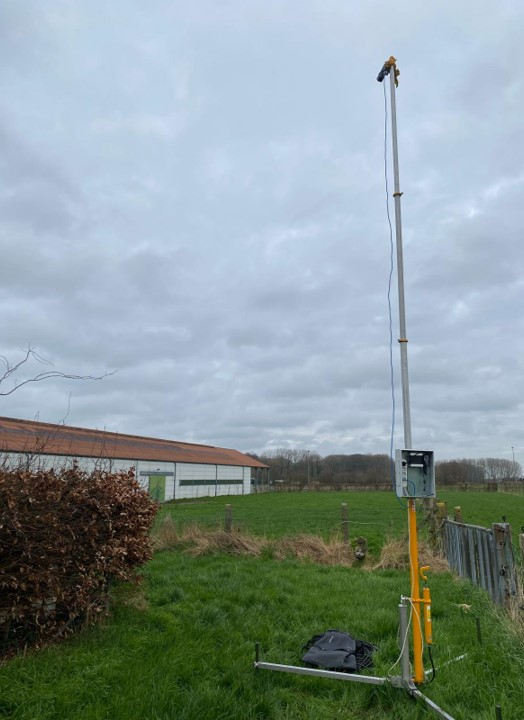
\includegraphics[width=0.5\linewidth]{datacollectie_paal.jpg}
  \caption{Opstelling van de camera voor het vastleggen van videomateriaal van koeien in een veld.}
  \label{fig:datacollectie_paal}  
\end{figure}
\section{Resultaten}
\begin{itemize}
  \item \textbf{Gelabelde Dataset:}  Aan het einde van deze fase werd een uitgebreide dataset verkregen die bestaat uit 3000 gelabelde frames met 5-6 koeien per frame. Deze dataset vormt de basis voor de ontwikkeling en het trainen van de objectdetectie- en gedragsclassificatiemodellen in de volgende fasen van de studie.
  \item \textbf{Datakwaliteit en -variabiliteit:} De kwaliteit en variabiliteit van de data werden verzekerd door de hoge resolutie van de opnamen en de diversiteit in gedrag en omgevingscondities, waardoor de modellen robuust en effectief zullen zijn onder verschillende omstandigheden.
\end{itemize}
\newline
\begin{figure}[H]
  \centering
  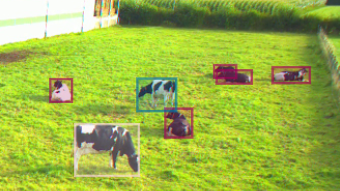
\includegraphics[width=\linewidth]{datacollectie_labeling.png}
  \caption{Resultaat van het labelingproces in Labelbox, waarbij bounding boxes en labels worden toegevoegd aan individuele frames van videomateriaal.}
  \label{fig:datacollectie_labeling}  
\end{figure}
\newline

\chapter{\IfLanguageName{dutch}{Ontwikkeling en Training van Objectdetectiemodellen}{Datacollection and Labeling}}%
\label{ch:objectdetectie}

\subsection{Doelstelling}
Deze fase was gericht op het ontwikkelen en trainen van geavanceerde objectdetectiemodellen om koeien en hun gedragingen nauwkeurig te identificeren binnen diverse agrarische omgevingen.

\subsection{Methoden}
\begin{itemize}
  \item \textbf{Voorbereiding van Data:}  De data geëxtraheerd uit Labelbox werd omgezet naar het YOLO dataformaat, wat noodzakelijk was om compatibiliteit met het modeltrainingsproces te verzekeren.
  \item \textbf{Modelselectie en Training:} Begonnen werd met het testen van verschillende YOLO-modellen. Er werd een voorgetraind YOLO-model gebruikt, gebaseerd op de COCO-dataset, om het trainingsproces te versnellen. 
  Deze modellen werden getraind op een rekencomputer uitgerust met 2 Nvidia A5000 GPU's van 25GB, wat een krachtige verwerkingscapaciteit bood voor het trainen van diepe neurale netwerken.
  Daarnaast werden een Faster R-CNN-model via Detectron en een SSD-model getest. Echter, het werd snel duidelijk dat YOLO-modellen eenvoudiger te gebruiken en op te zetten waren vanwege hun lagere complexiteit en eenvoudige implementatie. Bovendien leverden ze betere resultaten op dankzij de grote, voorgetrainde modellen die specifiek gericht zijn op objectdetectie, wat het hertrainen op aangepaste labels vergemakkelijkte.
  \item \textbf{Verfijning en Optimalisatie:} De focus verschoof naar verdere verfijning van de YOLO-modellen door verschillende parameters aan te passen en verschillende versies van YOLO te testen om de optimale configuratie te vinden voor de best mogelijke resultaten.
\end{itemize}

\subsection{Resultaten}
\begin{itemize}
  \item \textbf{Gekozen Model:}   Uiteindelijk werd gekozen om verder te gaan met het YOLO-model als de primaire keuze voor objectdetectie in dit onderzoek. Dit besluit was gebaseerd op de superieure prestaties en gebruiksgemak van het model in vergelijking met andere geteste modellen.
  \item 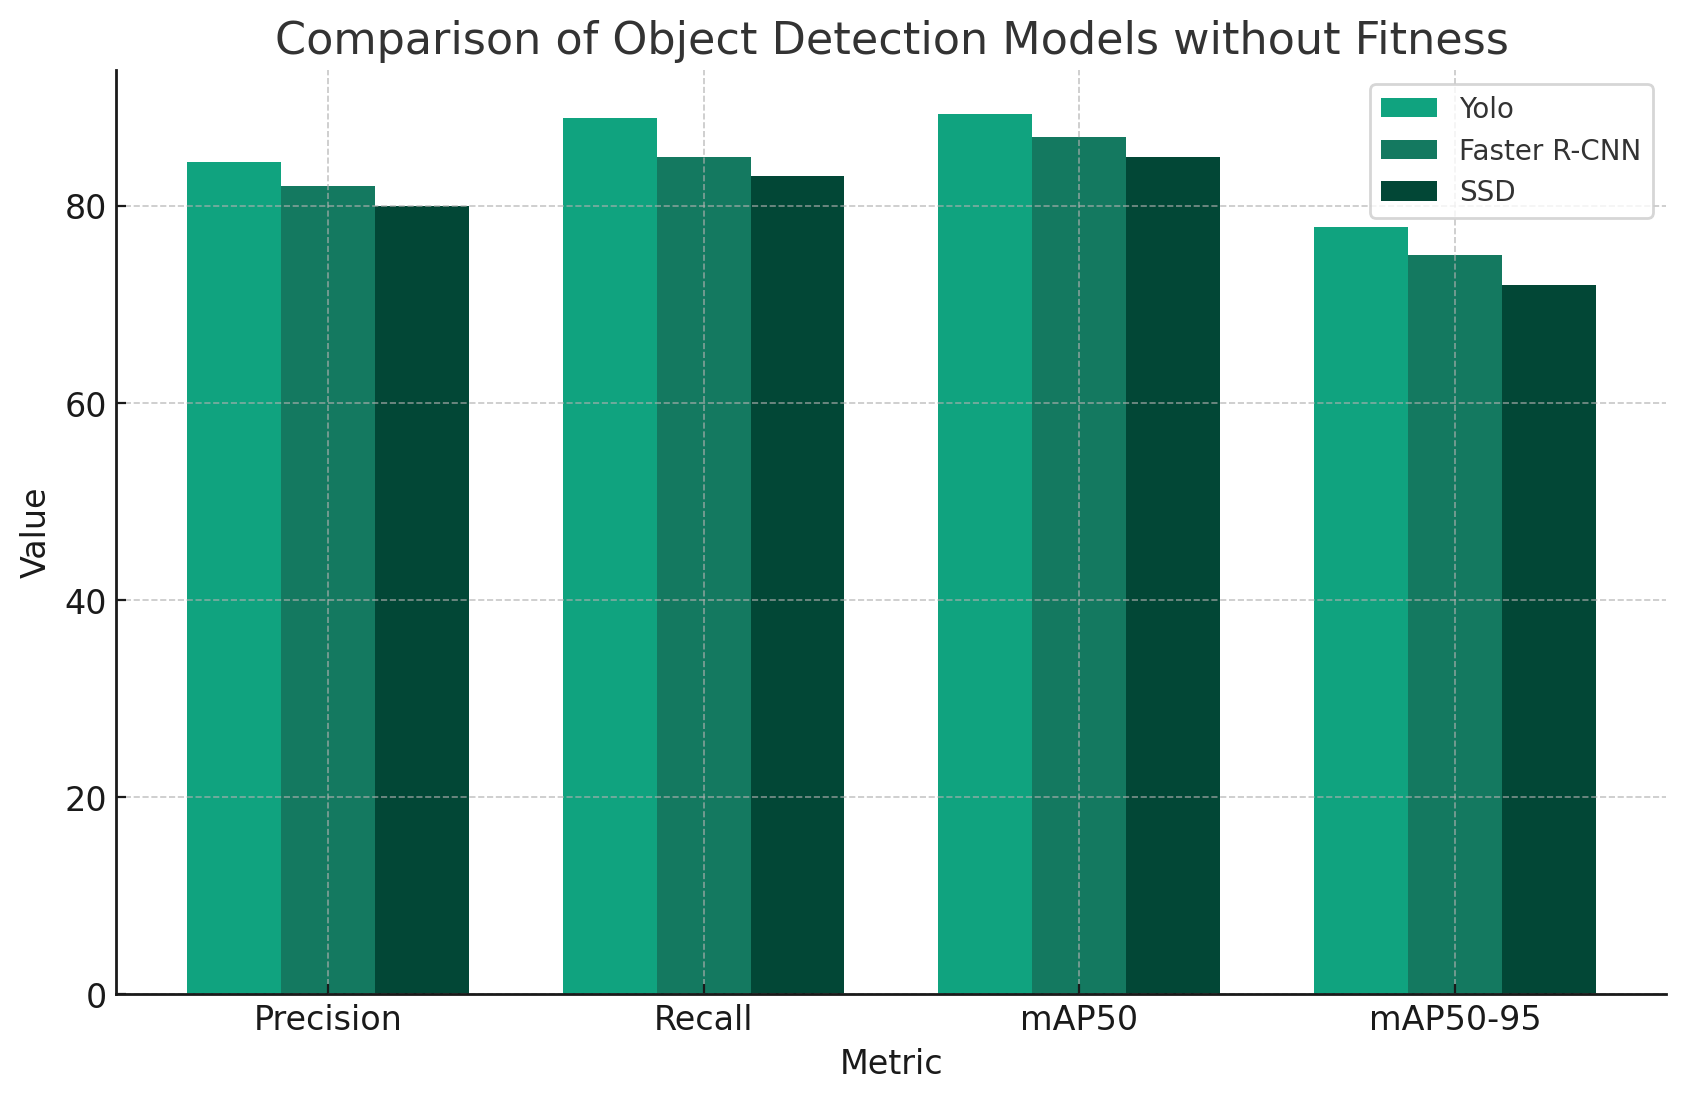
\includegraphics[width=\linewidth]{objectdetectie_metrics.png}
  \item \textbf{Modelprestaties:} Het geoptimaliseerde YOLO-model toonde duidelijke verbeteringen in het nauwkeurig detecteren en classificeren van koeiengedragingen, wat een robuust systeem opleverde dat effectief functioneerde binnen de complexe dynamiek van agrarische omgevingen.
\end{itemize}
\newline
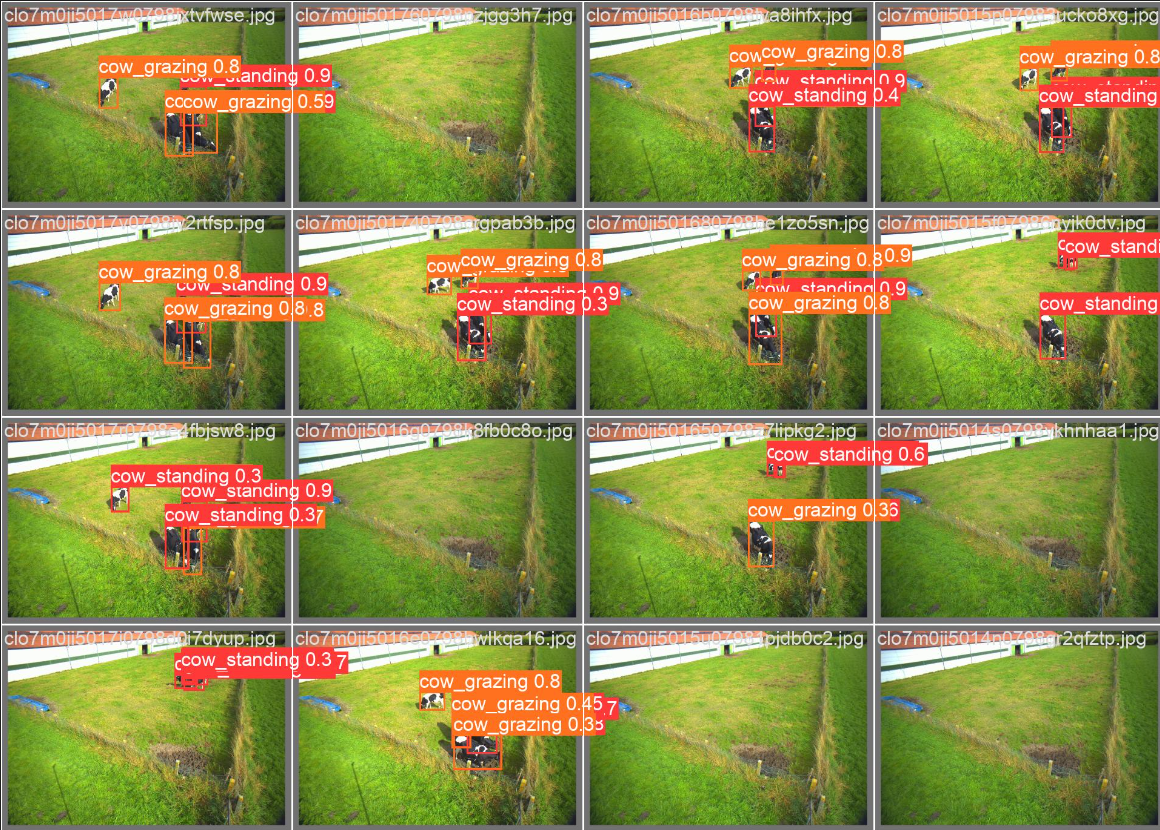
\includegraphics[width=\linewidth]{objectdetectie_yolo.png}
\newline
\chapter{\IfLanguageName{dutch}{Integratie van Voorgetrainde Pose Estimation Modellen}{Datacollection and Labeling}}%
\label{ch:poseestimation}

\subsection{Doelstelling}
Voor de pose estimation in dit onderzoek is gekozen voor het gebruik van het ViTPose model. Dit voorgetrainde model is bijzonder geavanceerd en staat bekend om zijn uitzonderlijke nauwkeurigheid en complexiteit in het identificeren van specifieke lichaamshoudingen. Het ViTPose model is specifiek ontworpen om uitdagingen in pose estimation te overwinnen door gebruik te maken van state-of-the-art technologieën en een omvangrijke trainingsdataset.

\subsection{Methoden}
\begin{itemize}
  \item \textbf{Trainingsdetails:} Voor de pose estimation is gekozen voor een voorgetraind ViTPose model, dat bekend staat om zijn hoge nauwkeurigheid en complexiteit. Dit model is getraind op de APT-36K dataset, een grootschalige dataset specifiek voor animal-pose estimation, bestaande uit 36,000 handmatig gelabelde foto's van 30 verschillende diersoorten. Het model identificeert 17 keypoints per dier, waaronder ogen, neus, nek, staart, schouders, ellebogen, knieën, heupen en poten. Het model is getraind op een indrukwekkende setup van 8 NVIDIA Tesla V100 (32G) GPUs. Deze krachtige GPU's bieden de noodzakelijke rekenkracht om grote en complexe datasets te verwerken, wat essentieel is voor de ontwikkeling van een robuust en nauwkeurig pose estimation model.
  \item \textbf{Alternatieve Trainingspogingen:} Er zijn experimenten uitgevoerd met voorgetrainde modellen op de COCO dataset en de APT10K dataset. Echter, uit deze tests bleek dat het model getraind op de APT-36K dataset de beste resultaten leverde voor de specifieke behoeften van dit onderzoek, vanwege de grotere variëteit en specialisatie in dierposes.
  \item \textbf{Beslissing tegen Eigen Training:} Gezien de complexiteit en de geavanceerde aard van het ViTPose model en de vereiste rekenkracht, werd besloten om het voorgetrainde model te gebruiken zonder verdere aanpassing of hertraining. Het zelf trainen van een dergelijk model zou niet alleen een vergelijkbare of betere dataset en vergelijkbare hardware vereisen, maar ook een diepgaande expertise in machine learning en computervisie. Bovendien is het onwaarschijnlijk dat een nieuw trainingsregime significant zou verbeteren op de reeds uitzonderlijke prestaties van het ViTPose model, gezien de kwaliteit en schaal van de initiële training.
  \item \textbf{Modelintegratie en Dataflow:} Eerst wordt objectdetectie uitgevoerd om de koeien in de videobeelden te identificeren en te lokaliseren. Voor elke gedetecteerde koe wordt een bounding box gecreëerd. Binnen deze bounding box gebruikt het ViTPose model de pose estimation technologie om de keypoints van het skelet van de koe te voorspellen.
  \item \textbf{Gedragsanalyse op Basis van Keypoints:} Specifieke algoritmes werden ontwikkeld om het gedrag van de koeien te interpreteren aan de hand van de posities van de keypoints. Bijvoorbeeld, de positie van de nek kan aangeven of een koe aan het grazen is, en de afstand tussen de heupen en poten kan aangeven of een koe ligt. Door de grootte van elke poot te berekenen ten opzichte van de lengte van de koe en de hoeken tussen elke poot en de nek te analyseren, kon gedrag nauwkeuriger worden vastgesteld dan met enkel objectdetectie.
\end{itemize}

\subsection{Resultaten}
\begin{itemize}
  \item \textbf{Integratie van Technologieën:} De integratie van objectdetectie en pose estimation modellen resulteerde in een krachtig systeem dat in staat is om gedetailleerd gedrag en lichaamshoudingen van koeien te analyseren.
  \item \textbf{Betrouwbaarheid van Gedragsclassificatie: } De combinatie van deze twee modellen verhoogt de betrouwbaarheid van de gedragsclassificatie aanzienlijk. Wanneer beide modellen hetzelfde gedrag suggereren, wordt de nauwkeurigheid van de classificatie effectief verhoogd naar een zeer hoog betrouwbaarheidsniveau.
  \item \textbf{Voorbeeld object detectie gedrag (links) vs pose estimation gedrag (rechts). } Duidelijk verbetering in gedrag voorspelling door diepere analyse van lichaamshoudingen met de pose estimation. 
  \newline 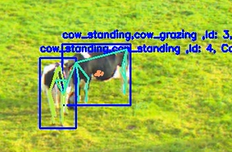
\includegraphics[width=\linewidth]{pose_werkend_voorbeeld.png}
  \item \textbf{Pretrained on COCO dataset:} \newline 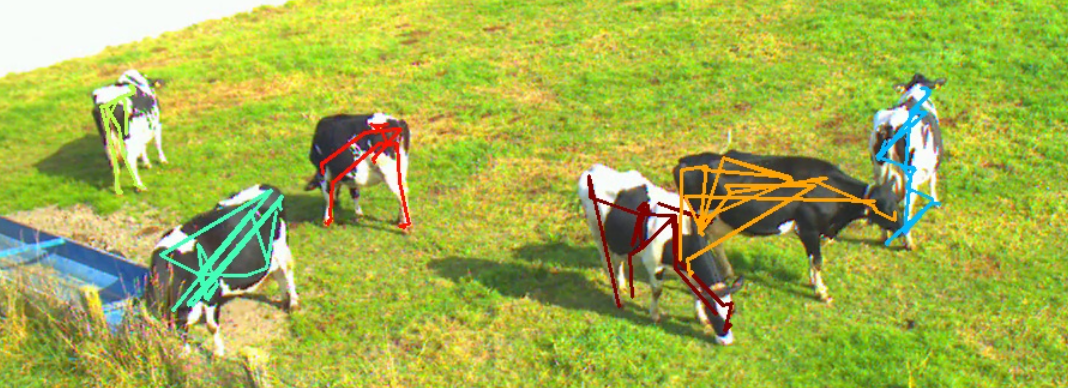
\includegraphics[width=\linewidth]{pose_cocoposes.png}
  \item \textbf{Pretrained on APT-36K dataset:} \newline 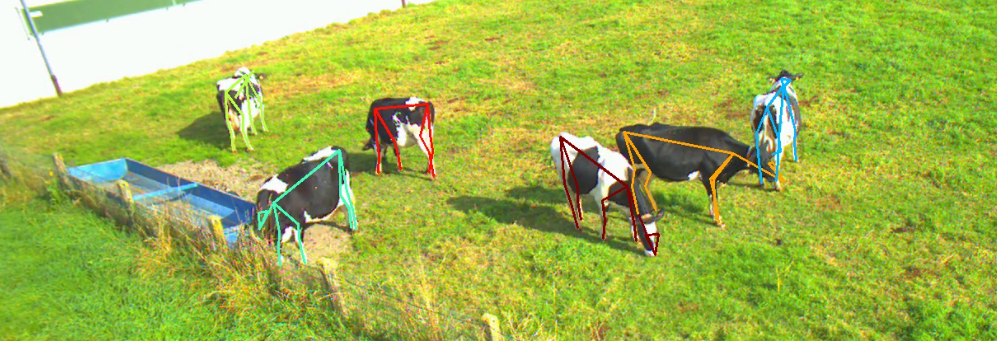
\includegraphics[width=\linewidth]{pose_apt36k.png}
\end{itemize}
\chapter{\IfLanguageName{dutch}{integratie van localisatie technologieën}{Integration of Localization Technologies}}%
\label{ch:localisatie}

\subsection{Doelstelling}
Deze fase was gericht op het integreren van geavanceerde locatietechnologieën om de exacte GPS-locaties van de koeien in het veld te bepalen door middel van cameraperspectieftransformatie. Het doel was om de nauwkeurigheid van de locatiegegevens te verhogen en real-time tracking van koeien op het veld mogelijk te maken.

\subsection{Methoden}
\begin{itemize}
  \item \textbf{Camera Perspective Transformation:}
  \begin{itemize}
    \item \textbf{Camera Intrinsics en Extrinsics:} Voor de implementatie van de locatiebepaling werd gebruik gemaakt van de intrinsieke (zoals de lensspecificaties) en extrinsieke (zoals de oriëntatie en positie ten opzichte van het veld) eigenschappen van de camera. Deze gegevens zijn essentieel voor het nauwkeurig omzetten van pixelcoördinaten in het beeld naar echte wereldcoördinaten op het veld.
    \item \textbf{Veld Kalibratie:} De vier hoeken van het veld werden in het camerabeeld gemarkeerd en gekoppeld aan de corresponderende GPS-locaties. Deze kalibratie maakte het mogelijk om de locatie van elk punt binnen het veld nauwkeurig te berekenen door de pixelpositie in het camerabeeld om te zetten naar een GPS-locatie.
  \end{itemize}
  \item \textbf{Nauwkeurigheidstests:}
  \begin{itemize}
    \item \textbf{Veldtests met een nepkoe:} Om de nauwkeurigheid van het systeem te verifiëren, werden experimenten uitgevoerd waarbij een nepkoe op verschillende locaties en in verschillende oriëntaties op het veld werd geplaatst. Voor elke positie werd de exacte GPS-locatie geregistreerd met behulp van een Emlid Reach Rs3 RTK GPS tracker, die bekend staat om zijn hoge nauwkeurigheid met een precisie tot op 1 cm in vaste positie.
    \newline 
    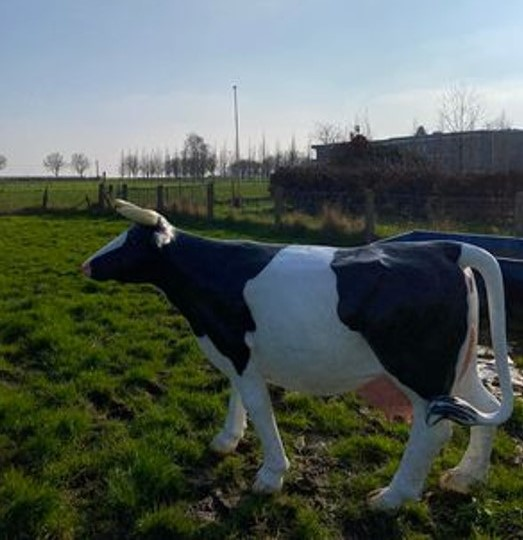
\includegraphics[width=0.7\linewidth]{localisatie_nepkoe.jpg}
    \newline 
    \item \textbf{Analyse van Foutmarges:} De initiële tests toonden een foutmarge van 0 tot 3 meter. Een consistente kleine foutmarge werd veroorzaakt door lichte bewegingen van de camera als gevolg van de wind. Deze fout bleek consistent in dezelfde richting te zijn, waardoor het mogelijk werd om de gemiddelde fout van de metingen af te trekken en zo de nauwkeurigheid van de camera-gebaseerde GPS-locaties te verbeteren tot een maximale foutmarge van 30 cm. Plannen voor het toepassen van beeldstabilisatie in de volgende fase zijn opgesteld om deze kleine bewegingen te compenseren.
    \item \textbf{Plot effectieve gps locaties:} 
    \newline 
    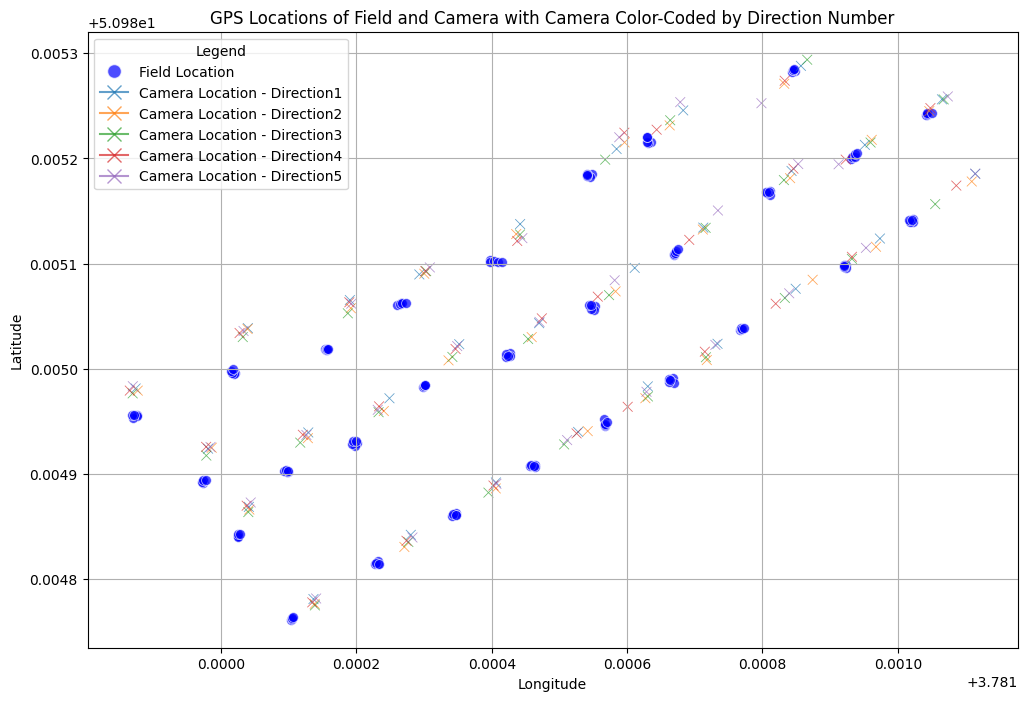
\includegraphics[width=\linewidth]{localisatie_plot_effectivelocations.png}
    \newline 
    \item \textbf{Plot gecorigeerde gps locaties:} 
    \newline
    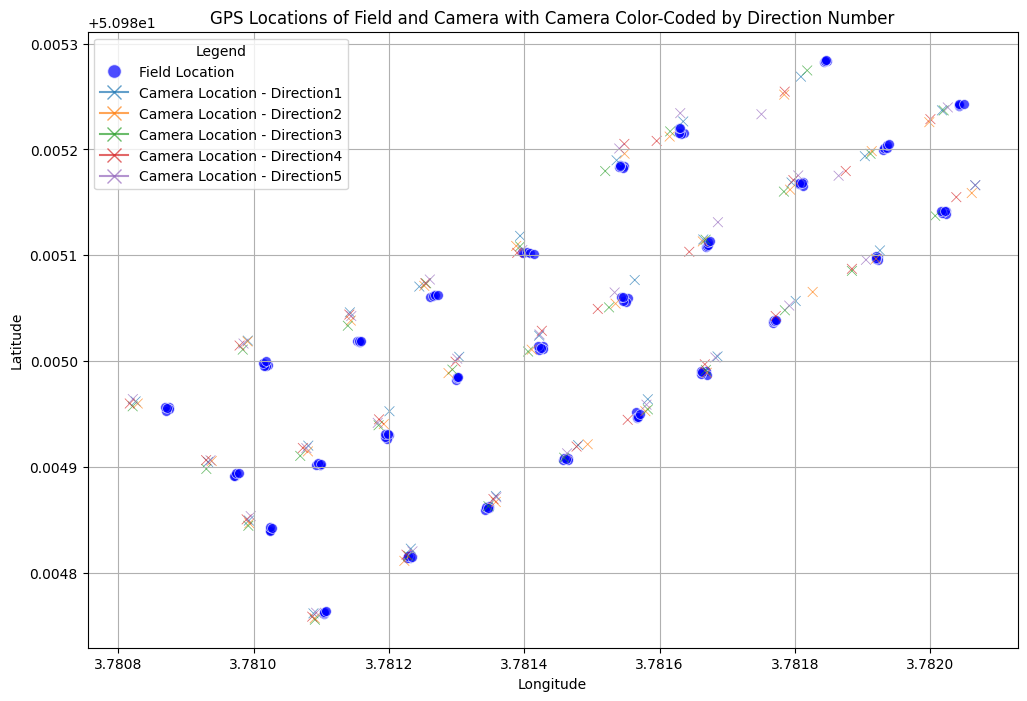
\includegraphics[width=\linewidth]{localisatie_plot_corrected_fault.png}
    \newline 
  \end{itemize}
\end{itemize}

\subsection{Resultaten}
\begin{itemize}
  \item \textbf{Geïmplementeerde Technologie:} De ontwikkelde techniek voor het bepalen van GPS-locaties via cameraperspectieftransformatie is succesvol geïmplementeerd en getest, wat heeft geleid tot een betrouwbare methode voor het real-time volgen van koeien op het veld.
  \item \textbf{Invloed van Rotatie:} Uit de analyses bleek dat de rotatie van de koe geen significante invloed had op de richting of afstand van de GPS-locaties, wat de robuustheid van het systeem bevestigt. 
  \newline 
  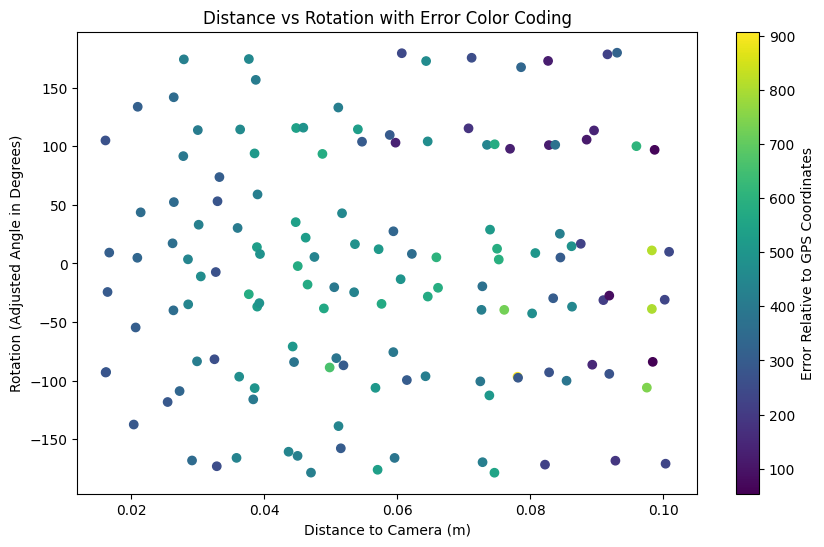
\includegraphics[width=\linewidth]{localisation_rotation_fault.png}
  \newline
  \item \textbf{Visualisatie en Evaluatie:} De resultaten van de locatiebepaling zijn gevisualiseerd en beoordeeld, waarbij de effectiviteit van de techniek werd bevestigd. Deze geavanceerde locatietechniek biedt aanzienlijke verbeteringen ten opzichte van traditionele niet-RTK GPS-sensoren, die doorgaans een foutmarge van ongeveer 3 meter hebben.
\end{itemize}
\chapter{\IfLanguageName{dutch}{Integratie van Beeldstabilisatie Technologieën}{Integration of Image Stabilization Technologies}}%
\label{ch:beeldstabilisatie}

\section{Doelstelling}
Deze fase was gericht op het implementeren van beeldstabilisatietechnieken om de effecten van camerabewegingen, veroorzaakt door externe factoren zoals wind, te minimaliseren. Het doel was om de kwaliteit van de videobeelden te verbeteren en daardoor de nauwkeurigheid van de locatiebepaling en gedragsanalyse van koeien te verhogen.

\section{Methoden}
\begin{itemize}
  \item \textbf{Voorbewerking van Frames:}
  \begin{itemize}
    \item \textbf{Omzetten naar Grijswaarden:} Elk videoframe werd eerst omgezet naar grijswaarden om de verwerkingssnelheid te verhogen en de complexiteit te verlagen.
    \item \textbf{Gaussische Blur:} Vervolgens werd een Gaussische filter toegepast om ruis in het beeld te verminderen, wat essentieel is voor de effectiviteit van de volgende stappen in de beeldverwerking.
    \item \textbf{Randdetectie met Canny-methode:} De randen in elk frame werden gedetecteerd met behulp van de Canny-methode, die helpt bij het identificeren van belangrijke structurele eigenschappen in de frames.
  \end{itemize}
  \item \textbf{Feature Detection en Mapping:}
  \begin{itemize}
    \item \textbf{Detectie van Kenmerkende Punten:} Met de Lucas-Kanade methode voor optische stroom werden kenmerkende punten binnen de frames gedetecteerd en gevolgd. Deze methode is effectief voor het volgen van bewegende objecten over opeenvolgende frames heen.
    \item \textbf{Schatten van de Affiene Transformatiematrix:} De verzamelde gegevens van de getrackte punten werden gebruikt om een affiene transformatiematrix te berekenen. Deze matrix beschrijft de nodige rotatie, schaling en translatie om het huidige frame uit te lijnen met de referentieframe.
  \end{itemize}
  \item \textbf{Toepassing van de Transformatie:}
  \begin{itemize}
    \item \textbf{Stabilisatie van de Videobeelden:} De berekende affiene transformatiematrix werd toegepast op elk frame om de videobeelden te stabiliseren. Dit proces corrigeert trillingen en andere ongewenste bewegingen van de camera, wat resulteert in een gladdere en visueel stabielere video-output.
  \end{itemize}
\end{itemize}

\section{Resultaten}
\begin{itemize}
  \item \textbf{Verbeterde Video Kwaliteit:} Door het toepassen van deze beeldstabilisatietechnieken werd een verbetering in de videokwaliteit bereikt. De gestabiliseerde beelden vertonen minder trillingen en zijn visueel aangenamer om naar te kijken.
  \item \textbf{Verhoogde Nauwkeurigheid van Data Analyse:} De stabilisatie van de videobeelden droeg bij aan de nauwkeurigheid van de geautomatiseerde analyses, zoals locatiebepaling en gedragsclassificatie, door consistente en duidelijke beelden te leveren die gemakkelijker te analyseren zijn.
\end{itemize}
\newline 
\begin{figure}[H]
  \centering
  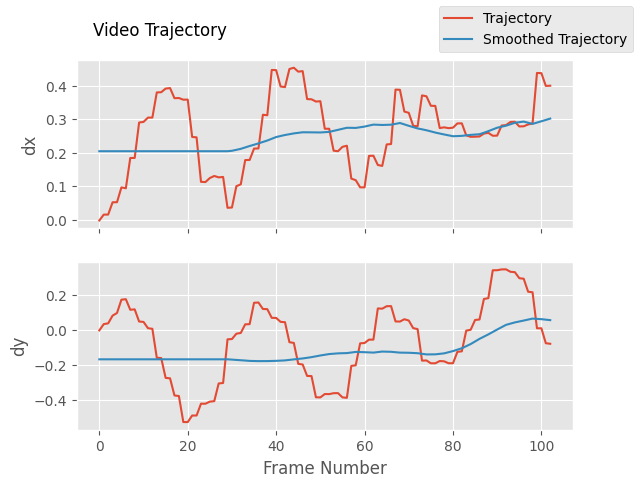
\includegraphics[width=\linewidth]{stabilisatie_traject.png}
  \caption{Grafiek van x en y traject van de video, voor en na beeldstabilisatie.}
  \label{fig:stabilisatie_traject}  
\end{figure}
\chapter{\IfLanguageName{dutch}{Algemene resultaten}{Results}}%
\label{ch:resultaten}

\subsection{Doelstelling}
Deze samenvatting presenteert de kernresultaten van het onderzoek uitgevoerd in de bachelorproef, gericht op de ontwikkeling van geavanceerde methoden voor de detectie en classificatie van koeiengedrag in een agrarische omgeving.

\section{Resultaten}
\subsection{Detectie en Classificatie van Koeiengedrag}
Het onderzoek heeft geleid tot de ontwikkeling van een robuust systeem dat in staat is om koeien te detecteren en hun gedrag in real-time te classificeren. Dit wordt gerealiseerd door video-opnamen gemaakt in het veld te analyseren met behulp van een geavanceerd machine learning model, de YOLOv8l. Dit model is specifiek getraind op een zorgvuldig samengestelde en gelabelde dataset, wat resulteert in snelle en accurate gedragsvoorspellingen. De belangrijkste voordelen van dit model zijn de hoge snelheid van beeldverwerking en de verminderde foutmarge in de gedragsclassificatie, cruciaal voor real-time monitoringtoepassingen.
\subsection{Analyse van Skelet-keypoints}
Deze sectie van het onderzoek onthult een van de meest innovatieve doorbraken: het gebruik van het ViTPose model. Dit model, dat is ontwikkeld met behulp van de uitgebreide APT-36K dataset, is geoptimaliseerd om de keypoints van het skelet van elke gedetecteerde koe nauwkeurig te identificeren. Deze keypoints zijn cruciaal, omdat ze gedetailleerde informatie verschaffen over de houding en bewegingen van de koeien.

De gegevens van de keypoints zijn niet alleen nuttig voor het in kaart brengen van de fysieke activiteiten van de koeien, maar zijn ook essentieel voor een diepgaande en gedetailleerde gedragsanalyse. Door nauwkeurig de bewegingen van specifieke lichaamsdelen te volgen, kunnen onderzoekers verfijnde inzichten verkrijgen in het natuurlijke gedrag van de koeien, zoals graaspatronen, rustposities, en interacties met andere koeien.

Bovendien speelt de precisie waarmee deze keypoints worden geïdentificeerd een cruciale rol bij het verifiëren en verbeteren van gedragsclassificaties. Wanneer de keypoints met een hoge mate van zekerheid worden vastgesteld, biedt dit een robuuste basis voor het algoritme om nauwkeurige gedragsclassificaties te maken. Dit is vooral van belang in situaties waar de gedragspatronen subtiel en complex zijn, en waar traditionele detectiemethoden mogelijk tekortschieten.

Het vermogen van het ViTPose model om geavanceerde analyses van koeiengedrag mogelijk te maken, opent nieuwe deuren voor het verbeteren van dierwelzijn en het efficiënt beheren van vee. Dit wordt bereikt door een beter begrip van hun gedragsbehoeften en -reacties op verschillende omgevingsfactoren, wat leidt tot meer gerichte en diervriendelijke managementstrategieën.
\subsubsection{Gedrag matches van pose vs classificatie}
98 procent matches tussen pose en classificatie van gedrag. Dit geeft een hoge mate van betrouwbaarheid aan in de voorspellingen van het systeem. 
Hieruit kan je ook conclusies trekken over de nauwkeurigheid van de pose estimation en de classificatie van gedrag, aangezien deze resultaten sterk overeenkomen.
\newline
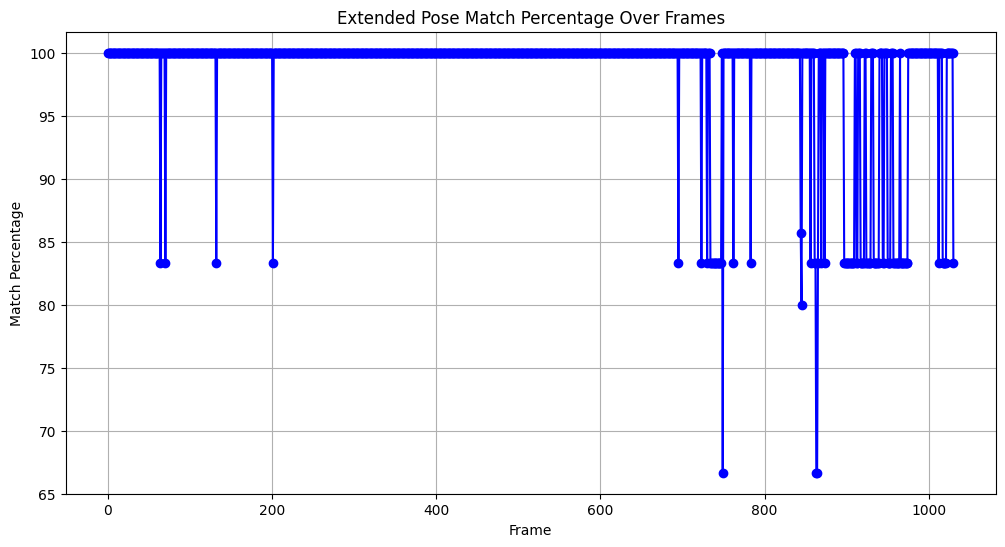
\includegraphics[width=\linewidth]{resultaten_pose_matches.png}
\newline
\subsubsection{Voorbeelden van betere gedragsclassificatie door pose estimation}
Deze afbeeldingen tonen de verbetering in gedragsclassificatie door de diepere analyse van lichaamshoudingen met de pose estimation. (links = classificatie gedrag, rechts = pose estimation gedrag)
\newline
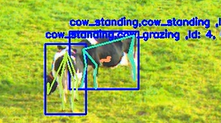
\includegraphics[width=\linewidth]{resultaten_verbetering_pose.png}
\newline
Deze afbeeldingen illustreren hoe de nauwkeurigheid van gedragsclassificatie afneemt door problemen met pose estimation, zoals een slechte positie van de koe. Mijn oplossing houdt in dat als de betrouwbaarheid van de keypoints te laag is, de voorspelling als onbetrouwbaar wordt beschouwd. In dat geval wordt het pose-gedrag niet voorspeld en blijft de oorspronkelijke gedragsclassificatie behouden.
\newline
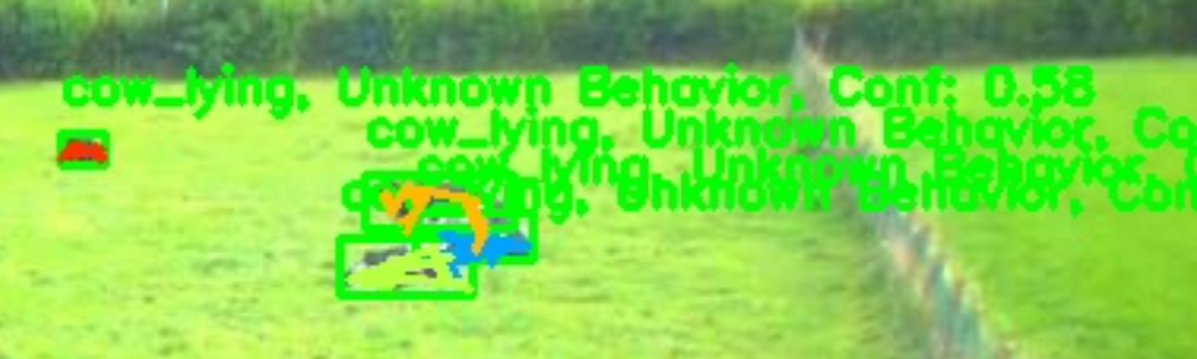
\includegraphics[width=\linewidth]{resultaten_slechte_pose_gedrag.png}
\newline
\subsection{Locatiebepaling via Cameraperspectieftransformatie}
De locatiebepaling van elke koe via cameraperspectieftransformatie vormt een innovatieve uitbreiding van het systeem. Deze techniek, die geavanceerde algoritmen gebruikt om de GPS-locatie van de koe te bepalen op basis van camerabeelden, verhoogt de nauwkeurigheid door integratie van beeldstabilisatietechnieken. Een belangrijk voordeel van deze methode is dat het de noodzaak elimineert om fysieke sensoren of GPS-apparaten direct op de koeien aan te brengen, wat bijdraagt aan een diervriendelijkere benadering van monitoring.

Deze techniek biedt niet alleen een diervriendelijk alternatief, maar verzekert ook continuïteit en betrouwbaarheid in de locatiedata, aangezien er geen risico is op uitval of defecten van sensoren die normaal gesproken op de koeien bevestigd zouden worden. Bovendien is deze methode bijzonder effectief in agrarische gebieden waar traditionele monitoringstechnieken zoals het gebruik van halsbanden of andere vormen van aan het dier bevestigde tracking niet haalbaar of wenselijk zijn.

Door gebruik te maken van deze cameragebaseerde locatiebepaling, kunnen boeren nauwkeurig de locatie en bewegingen van hun vee volgen zonder de welzijn van de dieren in gevaar te brengen. Dit leidt tot beter weidebeheer en geoptimaliseerde veebewegingsroutes, terwijl tegelijkertijd de gezondheid en het comfort van de koeien worden gewaarborgd. Deze aanpak ondersteunt niet alleen een effectiever beheer van het vee, maar bevordert ook een meer ethisch verantwoorde veehouderij.
\section{Conclusie}
De combinatie van deze technologieën biedt een nauwkeurige methode voor het lokaliseren en classificeren van het gedrag van koeien, wat een significante verbetering betekent voor het beheer en de monitoring van vee in de landbouw.
\newline
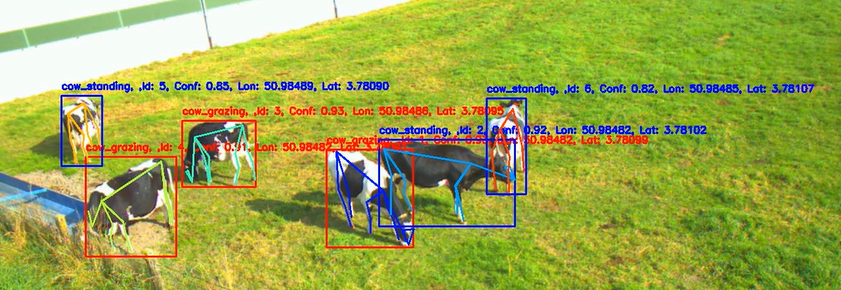
\includegraphics[width=\linewidth]{resultaten_alles.png}
\newline
\chapter{\IfLanguageName{dutch}{Mogelijk toekomstige uitbreidingen}{Future Research Possibilities}}
\label{ch:toekomst}
\subsection{Doelstelling}
Identificeren van potentiële gebieden voor verdere ontwikkeling en verbetering van de technologie, met als doel de nauwkeurigheid en functionaliteit van het koeiengedrag-detectiesysteem te verhogen.

\subsection{Geavanceerde Deep Learning Models voor Gedragsclassificatie}
Een kerngebied voor toekomstig onderzoek is de ontwikkeling van een geavanceerd diepgaand leermodel dat gedrag classificeert op basis van keypoints. Dit zou een verfijndere en contextueel nauwkeurigere analyse van koeiengedrag bieden, vergeleken met de huidige methoden die voornamelijk gebaseerd zijn op eenvoudige metingen van lichaamshoeken.

\subsection{Integratie van meerdere camera's}
Een andere significante verbetering zou de implementatie van meerdere camera's betreffen. Dit zou een breder en gedetailleerder beeld van de veeomgeving opleveren, waardoor het systeem effectiever koeien op grotere afstanden kan analyseren. Bovendien zou dit helpen bij het begrijpen van de sociale interacties en de ruimtelijke dynamiek binnen kuddes.

\subsection{Ontwikkeling van een Gespecialiseerde Keypoint Dataset}
Het creëren van een gespecialiseerde dataset met keypoints specifiek voor de koeien in de studie is een ander potentieel onderzoeksgebied. Dit zou de afhankelijkheid van algemene voorgetrainde modellen verminderen en de nauwkeurigheid van pose estimation significant verbeteren door deze te optimaliseren voor specifieke kenmerken van de onderzochte koeien.

\subsection{Uitbreiding van Gedragsclassificaties}
Het uitbreiden van gedragsclassificaties om nieuwe categorieën zoals sociale interacties en gezondheidsindicatoren te omvatten, zou een rijker begrip van koeienwelzijn bieden. Dit zou waardevolle inzichten verschaffen die gebruikt kunnen worden om veehouderijpraktijken te verbeteren, niet alleen door de fysieke, maar ook door de sociale en gezondheidsaspecten van koeien te adresseren.

Deze toekomstige onderzoeksrichtingen beloven niet alleen de technologische grenzen van diergedragsanalyse te verleggen maar bieden ook praktische voordelen voor de agrarische sector door een verbeterde monitoring en management van het vee.
% Voeg hier je eigen hoofdstukken toe die de ``corpus'' van je bachelorproef
% vormen. De structuur en titels hangen af van je eigen onderzoek. Je kan bv.
% elke fase in je onderzoek in een apart hoofdstuk bespreken.

%\input{...}
%\input{...}
%...

%%=============================================================================
%% Conclusie
%%=============================================================================

\chapter{Conclusie}%
\label{ch:conclusie}

% TODO: Trek een duidelijke conclusie, in de vorm van een antwoord op de
% onderzoeksvra(a)g(en). Wat was jouw bijdrage aan het onderzoeksdomein en
% hoe biedt dit meerwaarde aan het vakgebied/doelgroep? 
% Reflecteer kritisch over het resultaat. In Engelse teksten wordt deze sectie
% ``Discussion'' genoemd. Had je deze uitkomst verwacht? Zijn er zaken die nog
% niet duidelijk zijn?
% Heeft het onderzoek geleid tot nieuwe vragen die uitnodigen tot verder 
%onderzoek?

De locatiebepaling van elke koe via cameraperspectieftransformatie vormt een innovatieve uitbreiding van het systeem. Deze techniek, die geavanceerde algoritmen gebruikt om de GPS-locatie van de koe te bepalen op basis van camerabeelden, verhoogt de nauwkeurigheid door integratie van beeldstabilisatietechnieken. Een belangrijk voordeel van deze methode is dat het de noodzaak elimineert om fysieke sensoren of GPS-apparaten direct op de koeien aan te brengen, wat bijdraagt aan een diervriendelijkere benadering van monitoring.

Deze techniek biedt niet alleen een diervriendelijk alternatief, maar verzekert ook continuïteit en betrouwbaarheid in de locatiedata, aangezien er geen risico is op uitval of defecten van sensoren die normaal gesproken op de koeien bevestigd zouden worden. Bovendien is deze methode bijzonder effectief in agrarische gebieden waar traditionele monitoringstechnieken zoals het gebruik van halsbanden of andere vormen van aan het dier bevestigde tracking niet haalbaar of wenselijk zijn.

Door gebruik te maken van deze cameragebaseerde locatiebepaling, kunnen boeren nauwkeurig de locatie en bewegingen van hun vee volgen zonder de welzijn van de dieren in gevaar te brengen. Dit leidt tot beter weidebeheer en geoptimaliseerde veebewegingsroutes, terwijl tegelijkertijd de gezondheid en het comfort van de koeien worden gewaarborgd. Deze aanpak ondersteunt niet alleen een effectiever beheer van het vee, maar bevordert ook een meer ethisch verantwoorde veehouderij.



%---------- Bijlagen -----------------------------------------------------------

\appendix

\chapter{Onderzoeksvoorstel}

Het onderwerp van deze bachelorproef is gebaseerd op een onderzoeksvoorstel dat vooraf werd beoordeeld door de promotor. Dat voorstel is opgenomen in deze bijlage.

%% TODO: 
%\section*{Samenvatting}

% Kopieer en plak hier de samenvatting (abstract) van je onderzoeksvoorstel.

% Verwijzing naar het bestand met de inhoud van het onderzoeksvoorstel
%---------- Inleiding ---------------------------------------------------------

\section{Introductie}%
\label{sec:introductie}

In dit onderzoeksvoorstel, uitgevoerd bij ILVO, worden geavanceerde mogelijkheden van technologieën verkend voor het volgen en begrijpen van koeiengedrag in de moderne veehouderij. 
Het correct volgen en identificeren van gedrag van koeien is van cruciaal belang, niet alleen voor het welzijn van de dieren, maar ook voor de operationele efficiëntie van boerderijen. 
Deze studie richt zich op het analyseren van verschillende technologische methoden, waaronder objectdetectie en diepteschatting, om de locatie van koeien te bepalen en gedragingen zoals grazen, wandelen en rusten te identificeren. We onderzoeken de praktische uitdagingen en kansen die deze technologieën bieden in een agrarische omgeving. 
Het doel is om een diepgaand inzicht te krijgen in hoe deze technologische vooruitgang kan leiden tot verbeteringen in veehouderijpraktijken, met een specifieke focus op de impact op dierenwelzijn en boerderijbeheer. 
Dit onderzoek zal niet alleen bijdragen aan de wetenschappelijke kennis over diergedrag en technologische toepassingen in de landbouw, maar ook praktische richtlijnen bieden voor implementatie in de sector, wat de weg vrijmaakt voor innovatieve oplossingen in de toekomst van de landbouw.
%---------- Stand van zaken ---------------------------------------------------

\section{Literatuurstudie}%
\label{sec:state-of-the-art}
De technologische vooruitgang in de veehouderij heeft een nieuwe dimensie toegevoegd aan het volgen en analyseren van vee. 
De integratie van GPS- en RFID-technologieën, zoals onderzocht door \cite{Nääs2013} en \cite{Akhigbe2021}, heeft de basis gelegd voor efficiëntere trackingmethoden. 
Deze technologieën spelen een cruciale rol in het bieden van inzicht in de bewegingen en het gedrag van vee, wat essentieel is voor het beheer van hun gezondheid en welzijn.
Ontwikkelingen in computervisie en machine learning hebben nieuwe mogelijkheden geopend voor real-time monitoring en gedragsanalyse, zoals benadrukt door \cite{Kleanthous2018}. 
Geavanceerde technieken zoals objectdetectie en keypoints-analyse bieden gedetailleerde inzichten in het gedrag van vee, wat van groot belang is voor hun welzijnsbeoordeling. 
De toepassing van 3D-beeldvormings-technologieën, onderzocht \\door \cite{LeCozler2019}, heeft de precisie in het volgen en analyseren van vee verder verhoogd.
Deze methoden stellen ons in staat om gedetailleerde informatie te verzamelen, wat cruciaal is voor het beoordelen van de fysieke gezondheid van het vee.
Echter brengen deze ontwikkelingen ook uitdagingen met zich mee, zoals het identificeren van gedrag in verschillende omgevingscondities en het handhaven van nauwkeurigheid in complexe landbouwomgevingen \autocite{Narayan2023}\autocite{Busse2015}. 
Het is belangrijk om een evenwicht te vinden tussen het gebruik van geavanceerde technologieën en het waarborgen van dierenwelzijn en duurzaamheid.
Deze studies onderstrepen de vooruitgang en de voortdurende behoefte aan onderzoek en ontwikkeling in de implementatie en effectiviteit van technologieën. 
De integratie van deze technologieën belooft een efficiënte en diergerichte toekomst voor de veehouderij.
%---------- Methodologie ------------------------------------------------------
\section{Methodologie}%
\label{sec:methodologie}
Fasen van het onderzoek:
\begin{itemize}
  \item Fase 1: Literatuurstudie (2 week)
  \item Fase 2: Datacollectie (2 weken)
  \item Fase 3: Technologieën en Technieken (3 weken)
  \item Fase 4: Data-analyse en -verwerking (3 weken)
  \item Fase 5: Integratie en Evaluatie (2 weken)
  \item Fase 6: Conclusie (2 weken)
\end{itemize}
\subsection{Literatuurstudie}
Deze fase richt zich op het verkrijgen van een kennis van de huidige stand van zaken in de technologieën voor vee tracking. 
De focus ligt op het analyseren van studies over machine learning en computervisie. 
Hierbij is het doel het identificeren van de meest effectieve methoden en technieken voor gedragsanalyse van vee.
\end{itemize}
\subsection{Datacollectie}
In deze fase richt het onderzoek zich op de collectie van real-time gedragsdata van koeien met behulp van camera's. 
Het doel is om methoden voor data-extractie en -beheer te verkennen en te analyseren. 
De focus ligt op het opzetten van geautomatiseerde data pipelines, terwijl tegelijkertijd de bestaande technologieën en datasets van ILVO worden onderzocht. 
Dit onderzoek zal bepalen of en hoe ILVO's huidige middelen kunnen bijdragen aan de verrijking en uitbreiding van de verzamelde data. 
Elke stap in dit proces zal worden onderbouwd met zorgvuldig onderzoek, om te verzekeren dat de aanpak zowel wetenschappelijk gefundeerd als praktisch haalbaar is.
\end{itemize}
\subsection{Technologieën en Technieken}
De focus van dit onderdeel is de selectie en integratie van de meest geschikte technologieën voor de gedetailleerde analyse van koeiengedrag.
Dit proces omvat de aanpassing en toepassing van diverse bestaande computervisietechnieken.
  \begin{itemize}
    \item Objectdetectie: We zullen geavanceerde object-
    detectie-algoritmen zoals YOLO, SSD en Faster R-CNN inzetten. Deze technieken zijn cruciaal voor het nauwkeurig identificeren en lokaliseren van koeien binnen videobeelden, wat de basis vormt voor verdere gedragsanalyse.
    \item Keypoints-analyse: Voor de gedetailleerde analyse van bewegingen en houdingen van koeien, zullen keypoints-analyse technieken zoals OpenPose en AlphaPose worden gebruikt. Deze technieken stellen ons in staat om specifieke punten op het lichaam van de koe te identificeren en te volgen, wat essentieel is voor het begrijpen van hun gedrag.
    \item Bewegingsanalyse: Door de toepassing van optische stroming en tracking-algoritmen kunnen we de bewegingen van koeien over tijd volgen. Dit helpt ons om patronen in hun beweging te herkennen en te analyseren.
    \item Gedragsclassificatie: Machine learning en deep learning technieken zullen worden gebruikt voor de classificatie van specifieke gedragingen. Dit stelt ons in staat om verschillende gedragspatronen te identificeren en te categoriseren, van eenvoudige acties tot complexe sociale interacties.
    \item Anomaliedetectie: Tot slot zullen we anomalie
    detectie-technieken inzetten om afwijkingen van normaal gedrag te identificeren, wat kan wijzen op gezondheidsproblemen of stress bij de koeien.
  \end{itemize}
Deze geïntegreerde aanpak combineert meerdere computervisietechnieken om een uitgebreid en nauwkeurig beeld te krijgen van het gedrag van koeien. De keuze voor specifieke technologieën en de integratiestrategie zal worden onderbouwd door uitgebreid onderzoek en analyse, om de effectiviteit en nauwkeurigheid van de gedragsanalyse te maximaliseren.
\end{itemize}
\subsection{Data-analyse en -verwerking}
In de data-analyse en -verwerkingsfase van de bachelorproef wordt gebruik gemaakt van geavanceerde machine learning algoritmen om koeiengedrag te analyseren en te classificeren.
De focus ligt op de volgende aspecten:
  \begin{itemize}
    \item Selectie van Algoritmen: We zullen specifieke machine learning algoritmen kiezen die het best passen bij onze data en analysebehoeften. Dit kan variëren van Convolutional Neural Networks (CNNs), die effectief zijn voor beeldclassificatie en herkenning, tot Recurrent Neural Networks (RNNs) die geschikt zijn voor het analyseren van tijdsafhankelijke data. Afhankelijk van de complexiteit van de gedragspatronen, kunnen ook eenvoudigere algoritmen zoals Decision Trees of Support Vector Machines (SVMs) worden overwogen.
    \item Training en Optimalisatie: Zodra de algoritmen zijn geselecteerd, worden deze getraind met de verzamelde data. Dit proces omvat het afstellen van parameters en het toepassen van technieken zoals cross-validation om de effectiviteit van de modellen te maximaliseren.
    \item Validatie: Na het trainen van de modellen is het essentieel om hun prestaties te testen en valideren met nieuwe, ongeziene data. Dit helpt ons om de nauwkeurigheid en betrouwbaarheid van de modellen te beoordelen.
  \end{itemize}
Deze aanpak zorgt ervoor dat we diepgaande en betrouwbare inzichten verkrijgen in koeiengedrag, ondersteund door robuuste data-analyse en \\-verwerkingstechnieken.
\end{itemize}
\subsection{Integratie en Evaluatie}
Implementatie en toetsing van de ontwikkelde technieken en modellen in een realistische landbouwomgeving. 
Beoordeling van de effectiviteit, nauwkeurigheid en bruikbaarheid van de technologieën. 
\subsection{Conclusie}
Reflectie op de resultaten van het onderzoek, met een nadruk op de impact van de geïntegreerde technologieën en methoden op de veehouderijpraktijk. 
Aanbevelingen voor toekomstig onderzoek en mogelijke verbeteringen.
\subsection{Gantt-chart}
\newline
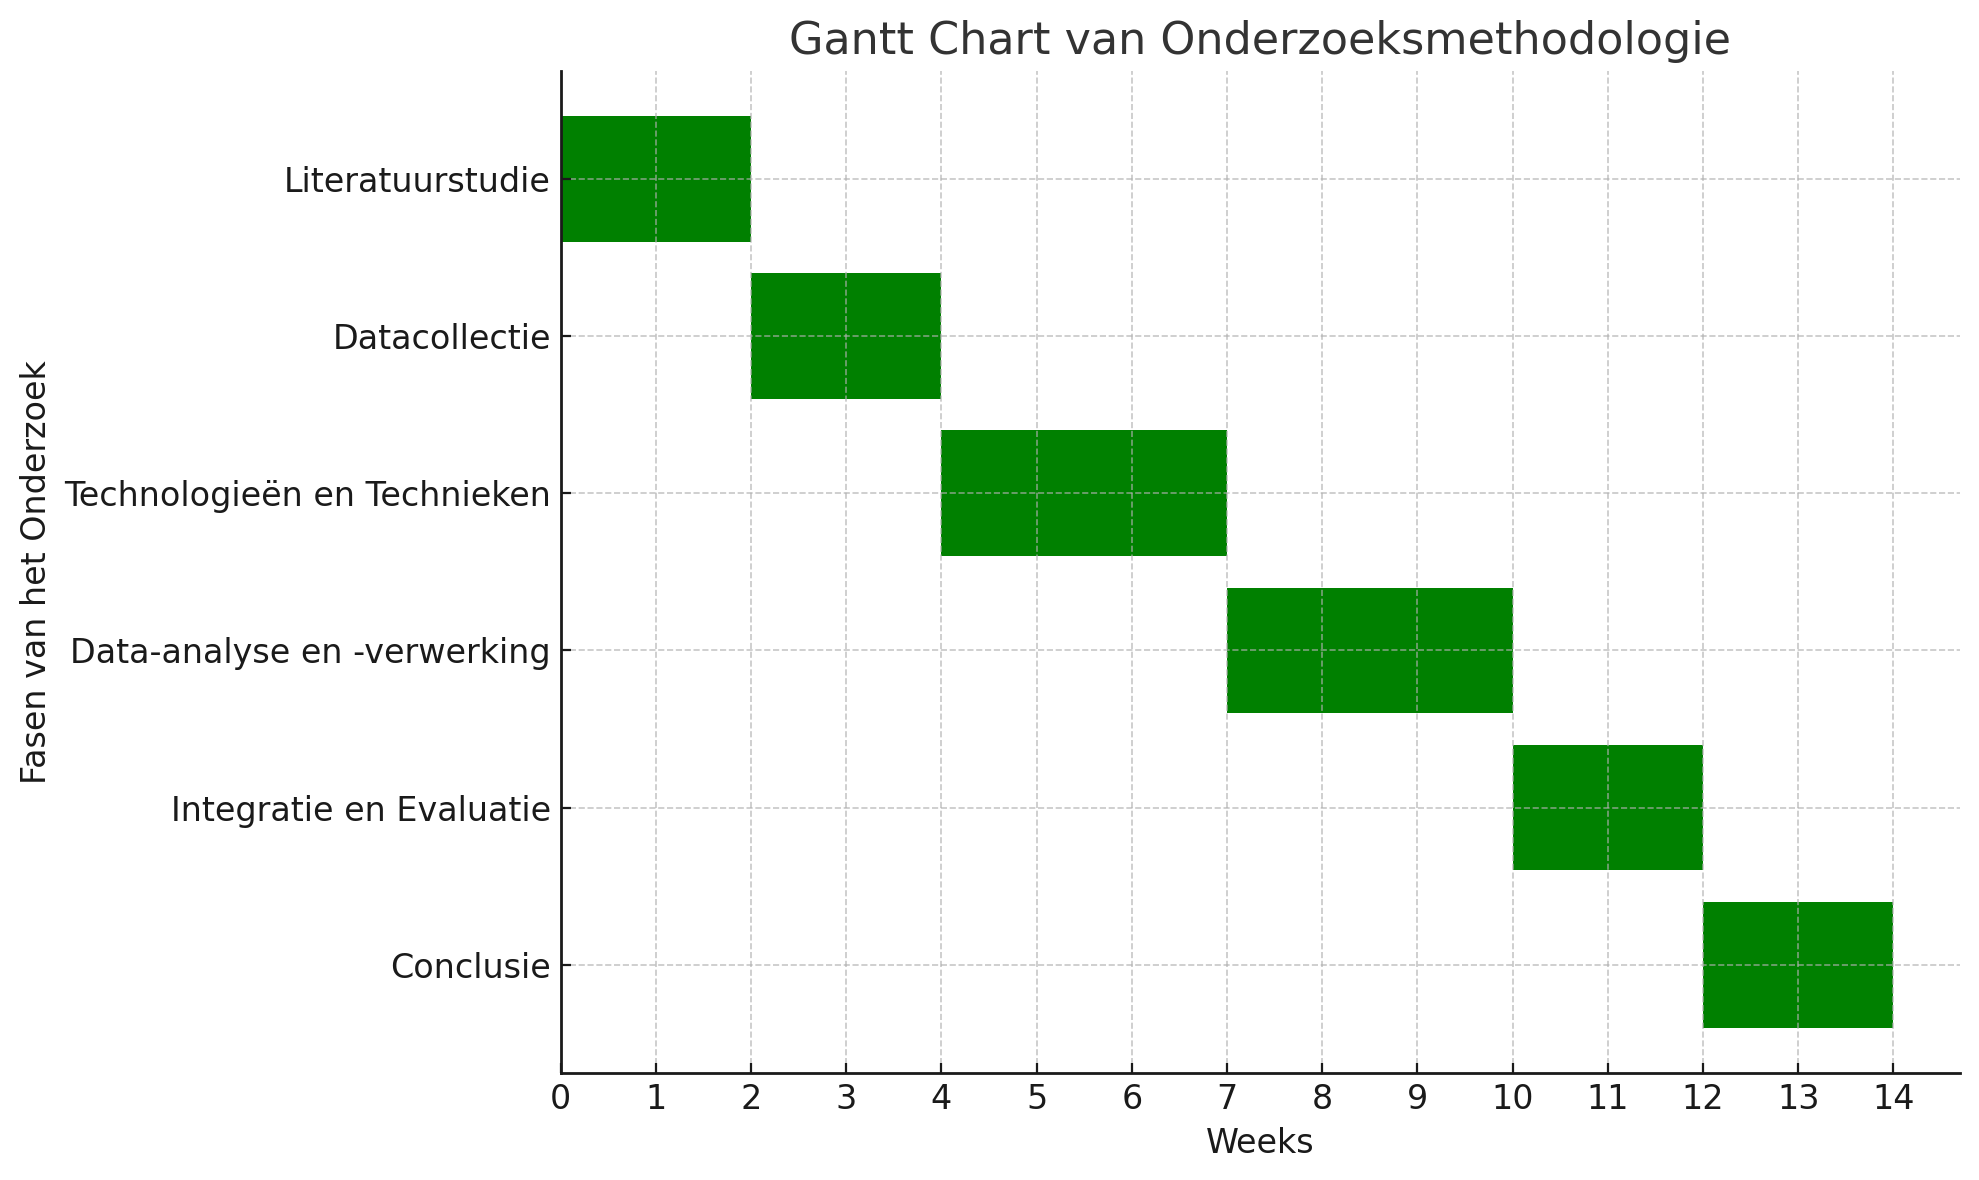
\includegraphics[width=\linewidth]{gantt_chart.png}
\newline
%---------- Verwachte resultaten ----------------------------------------------
\section{Verwacht resultaat, conclusie}%
\label{sec:verwachte_resultaten}
In dit onderzoek verwachten we de volgende resultaten te verkrijgen:
\begin{itemize}
  \item Verbeterde nauwkeurigheid in het monitoren van koeiengedrag door geavanceerde technologieën, zoals objectdetectie en \newline keypoints-analyse, toe te passen.
  \item Efficiëntere methoden voor gedragsanalyse van koeien in verschillende omgevingsomstandigheden.
  \item Geavanceerde Analytische Inzichten: In plaats van een geïntegreerd systeem voor locatie- en gedragsvolging, zal de focus liggen op het ontwikkelen van geavanceerde analytische inzichten die de basis leggen voor toekomstige integratie in dergelijke systemen. Het doel is om diepgaande kennis te verwerven over koeiengedrag, wat cruciaal is voor het ontwerpen van effectieve monitoringssystemen.
\end{itemize}
Deze resultaten zullen een meerwaarde bieden voor de veehouderij door bij te dragen aan het welzijn van dieren en de operationele efficiëntie te verbeteren. Het gebruik van geavanceerde technologieën voor gedragsmonitoring kan leiden tot betere besluitvorming en zorg voor het vee, en uiteindelijk tot positieve economische en ethische gevolgen voor de landbouwsector.

Het is belangrijk op te merken dat de uiteindelijke resultaten kunnen variëren op basis van de uitkomsten van de data-analyse en evaluatie van de gebruikte technologieën. 
Dit onderzoek zal een grondige analyse bieden om eventuele afwijkingen te verklaren en aanbevelingen te doen voor verdere verbeteringen.


%%---------- Andere bijlagen --------------------------------------------------
% TODO: Voeg hier eventuele andere bijlagen toe. Bv. als je deze BP voor de
% tweede keer indient, een overzicht van de verbeteringen t.o.v. het origineel.
%\input{...}

%%---------- Backmatter, referentielijst ---------------------------------------

\backmatter{}

\setlength\bibitemsep{2pt} %% Add Some space between the bibliograpy entries
\printbibliography[heading=bibintoc]

\end{document}
